\chapter{Network Training}
\section{Backpropagation in Neural Networks}


\begin{figure}[H]
    \centering
    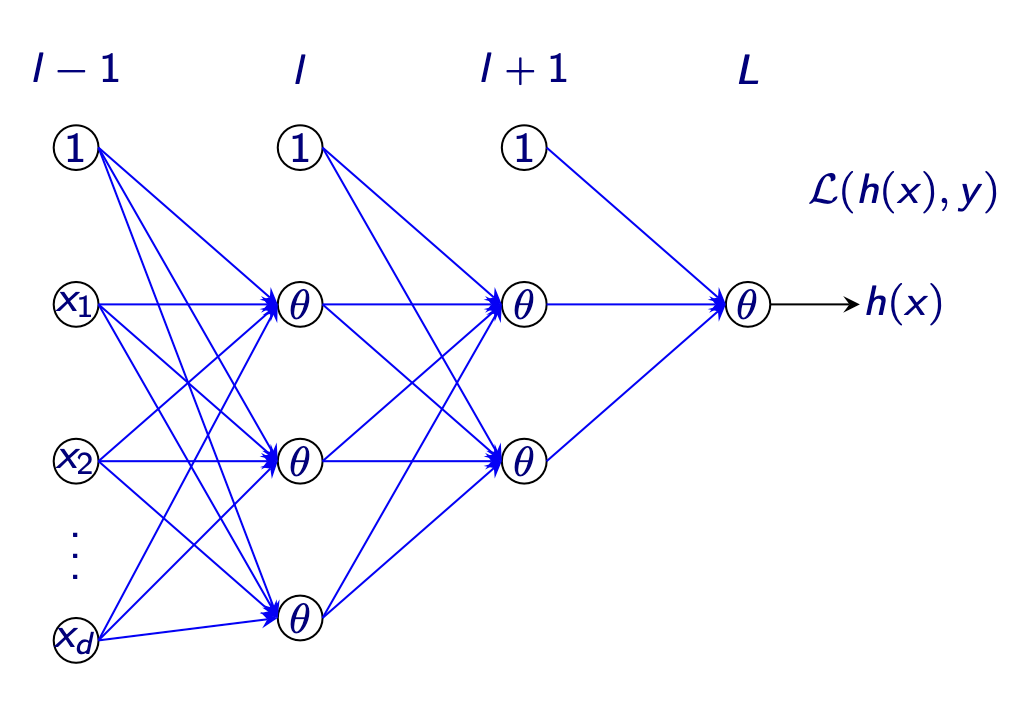
\includegraphics[width=0.55\linewidth]{img/nn.png}
\end{figure}

\begin{itemize}
    \item \textbf{Weights} are denoted as \( W^{(l)} \) for layer \( l \), with \( W_{ij}^{(l)} \) representing the weight from the \( i \)-th neuron in layer \( l-1 \) (input) to the \( j \)-th neuron in layer \( l \) (output). The layer indexing runs from 1 to \( L \) where \( L \) is the total number of layers.
    \item The \textbf{input} vector \( x \) applied to the input layer, represented as \( x^{(0)} \) with components \( x_1^{(0)}, \ldots, x_{d^{(0)}}^{(0)} \), leads to the output \( x_1^{(L)} = h(x) \in \mathbb{R} \), where \( h(x) \) is the hypothesis function.
    \item \textbf{Activations} (outputs) of layer \( l \) are denoted as \( x_j^{(l)} \), which are computed using an activation function \( \theta \) applied to the pre-activation values \( s_j^{(l)} \). This can be expressed as:
    \[ x_j^{(l)} = \theta(s_j^{(l)}) = \theta \left( \sum_{i=0}^{d^{(l-1)}} W_{ij}^{(l)} x_i^{(l-1)} \right) \]
    where \( d^{(l-1)} \) and \( d^{(l)} \) are the number of inputs and outputs for layer \( l \), respectively.
    \item The \textbf{diagonal matrix of activations} at layer \( l \), denoted as \( \Theta^{(l)} \), is the diagonal matrix containing the activation function derivatives and can be calculated as:
    \[ \Theta^{(l)} = \text{diag}(\theta'(s^{(l)})) \]
    which is a square matrix with dimensions equal to the number of outputs of layer \( l \).
    \item The \textbf{gradient} with respect to the pre-activation values \( s^{(l)} \) is given by \( \delta^{(l)} \), which is used in the backpropagation algorithm to compute the gradient of the loss function with respect to the weights \( W^{(l)} \).
\end{itemize}


\begin{definitionbox}{Gradient}
The gradient \( \delta^{(l)} \) for layer \( l \) in a neural network during backpropagation is given by:
\[ \delta^{(l)} = \left( \prod_{k=l}^{L-1} \Theta'(s^{(k)})W^{(k)T} \right)\Theta'(s^{(L)}) \nabla_{x^{(L)}} \mathcal{L} \]
where \( \Theta'(s^{(l)}) \) is the derivative of the activation function evaluated at the pre-activation level \( s^{(l)} \), \( W^{(k)} \) are the weights of layer \( k \), and \( \nabla_{x^{(L)}} \mathcal{L} \) is the gradient of the loss \( \mathcal{L} \) with respect to the activations of the last layer \( x^{(L)} \).

The update rule for the weights is then:
\[ \Delta W^{(l)} = \nabla_W \mathcal{L} = -\eta x^{(l-1)} \delta^{(l)} \]
which includes the learning rate \( \eta \), and requires forward propagation to obtain the error \( \mathcal{L} \).
\end{definitionbox}

\section{The Problem of Vanishing and Exploding Gradients}

The vanishing and exploding gradient problem is a significant challenge in training deep neural networks. It occurs during backpropagation, described as:
\[ \delta^{(l)} = \left( \prod_{k=l}^{L-1} \Theta'(s^{(k)})W^{(k)T} \right)\Theta'(s^{(L)}) \nabla_{x^{(L)}} \mathcal{L} \]
where \( \delta^{(l)} \) represents the gradient at layer \( l \), \( \Theta'(s^{(k)}) \) is the derivative of the activation function at the pre-activation values \( s^{(k)} \), and \( W^{(k)} \) is the weight matrix for layer \( k \).

\begin{itemize}
    \item Activation functions like sigmoid or tanh can saturate, which means their derivatives can become very small. Consequently, during backpropagation, these small derivatives multiply together exponentially with depth, leading to very small gradients. This is known as the \textbf{vanishing gradient} problem, which results in slow or stagnant learning.
    \item On the other hand, if the weight matrices have large eigenvalues, the gradients can grow exponentially as they backpropagate through the layers, leading to the \textbf{exploding gradient} problem, where weight updates are so large they can cause the learning process to diverge.
    \item Deep networks are particularly susceptible to these issues due to their depth and complexity.
\end{itemize}

\subsection*{Intuitive Explanation}
Consider the backpropagation of errors in a deep network as a process of transmitting signals. If the transmission channel (represented by the activation functions and weight matrices) weakens the signal too much (vanishing gradients), the information about the error doesn't reach the earlier layers effectively. This is similar to whispering a message across a long chain of people– by the time it reaches the end, the message might be lost.\\

Conversely, if the channel amplifies the signal too much (exploding gradients), the information about the error overshoots its target, leading to large, erratic updates. This is akin to using a megaphone for the same message in a small room; the message doesn't just reach the intended person but bounces around the walls, creating chaos.

\subsection*{Mitigation Strategies}
To address these problems, several strategies are employed:
\begin{itemize}
    \item \textbf{Network Design:} Architectural choices, such as using shorter connections (skip connections) that allow gradients to bypass certain layers directly.
    \item \textbf{Initialisation:} Careful initialisation of the weights to ensure that the eigenvalues of the weight matrices are neither too small nor too large.
    \item \textbf{Regularisation:} Techniques such as gradient clipping are used to prevent gradients from becoming too large.
\end{itemize}


\begin{definitionbox}{Epoch}
An \textbf{Epoch} represents a single pass through the entire dataset, where each example in the dataset has been used once for both forward and backward propagation. Typically, a single epoch is not sufficient for convergence; the model may require multiple epochs to adequately learn from the data. As the number of epochs increases, the model's performance on training data usually improves, from underfitting to optimal fitting, and can eventually lead to overfitting. The appropriate number of epochs can vary widely between different datasets.
\end{definitionbox}

\begin{definitionbox}{Batch}
A \textbf{Batch} refers to the subset of the dataset that is processed together in one iteration of training. The entire dataset is divided into a number of these batches. The \textbf{Batch Size} is the number of training examples in a single batch. It is important to distinguish between batch size and the number of batches, which are related but not the same—the number of batches is determined by dividing the total number of examples by the batch size.
\end{definitionbox}

\begin{definitionbox}{Iteration}
An \textbf{Iteration} is one update of the model's parameters, which is done after processing a batch. The number of iterations needed to complete one epoch is equal to the number of batches in the dataset. Therefore, the number of iterations for one epoch is the total number of examples divided by the batch size.
\end{definitionbox}

\section{Reducing Overfitting}

There are several measures we can take to reduce overfitting in models. This is usually because the network is too large, it has been trained too long on the data, or a lack of data points.

\subsection*{Remedies}
\begin{itemize}
    \item Reduce network complexity, less layers
    \item Regularisation 
        \begin{itemize}
            \item Momentum and weight decay
            \item Dropout
            \item Weight initialisation
            \item Batch normalisation
        \end{itemize}
    \item Data augmentation
    \item Patience/early stopping
    \item Weight sharing
    \item Ensemble predictions (pattern recognition)
    \item Multitask learning
    \item Adversarial training (hard negatives)
\end{itemize}

\section{Optimisers}
\begin{commentbox}{Notation: Hadamard Product}
    We use \(\odot\) to refer to the Hadamard product, which consists of element-wise multiplication. The Hadamard product is associative and distributive. Unlike the matrix product, it is also commutative.

    \[
\begin{bmatrix}3&5&7\\4&9&8\end{bmatrix}\odot\begin{bmatrix}1&6&3\\0&2&9\end{bmatrix}=\begin{bmatrix}3\times1&5\times6&7\times3\\4\times0&9\times2&8\times9\end{bmatrix}
    \]
    
\end{commentbox}
\subsection{Stochastic Gradient Descent (Mini batch)}

\begin{definitionbox}{Mini-batch Stochastic Gradient Descent (SGD)}
Mini-batch Stochastic Gradient Descent (SGD) is an optimisation technique used to train neural networks by updating the model's weights based on the gradient of the loss function with respect to the weights. Key components of mini-batch SGD include:

\begin{itemize}
    \item \textbf{Loss Function}: The average loss over a mini-batch is given by
    \[ \mathcal{L} = \frac{1}{n} \sum_{i} \ell(h(x_i), y_i) \]
    where \( \ell \) is the loss for a single data point, \( h(x_i) \) is the hypothesis function evaluated at input \( x_i \), and \( y_i \) is the true label.

    \item \textbf{Gradient of the Loss}: The gradient with respect to the weights \( W \) is
    \[ \nabla_W \mathcal{L} = \frac{1}{n} \sum_{i} \nabla_W \ell(h(x_i), y_i) \]

    \item \textbf{Weight Update}: The weights are updated by moving in the negative direction of the gradient, scaled by the learning rate \( \eta \):
    \[ W_{t+1} = W_t - \eta \nabla_W \mathcal{L}_t \]

    \item \textbf{Learning Rate \( \eta \)}: This hyperparameter controls the step size during the weight update. It plays a crucial role in convergence and must be carefully tuned. A learning rate that is too high can cause the training to diverge, while a rate that is too low results in slow convergence.

    \begin{figure}[H]
    \centering
    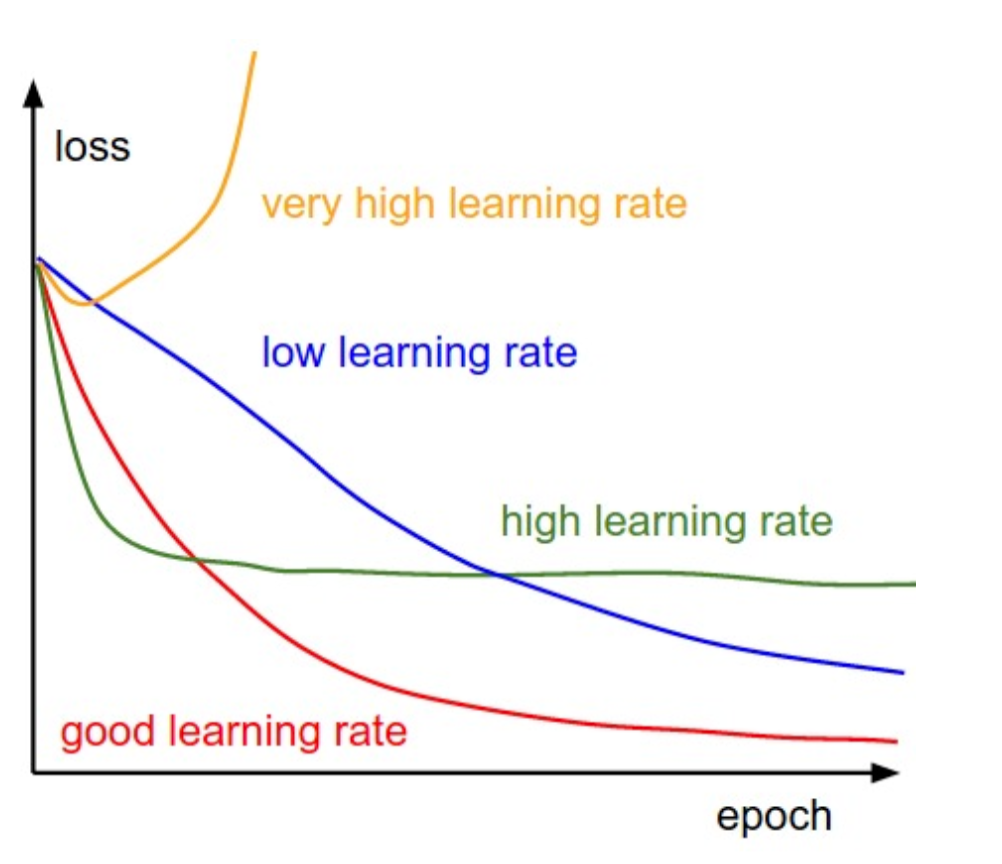
\includegraphics[width=0.5\linewidth]{img/sgd_learnrate.png}
    \caption{Graph showing a loss over epochs for different learning rates}
    \end{figure}
\end{itemize}

Convergence can be slow with mini-batch SGD, and selecting an appropriate learning rate often requires experimentation. Learning rate schedules or adaptive learning rate methods are used to adjust \( \eta \) during training to improve convergence.
\end{definitionbox}



\begin{definitionbox}{SGD with momentum (mini-batch)}


SGD with momentum is a variation of the standard SGD that accelerates convergence by incorporating a fraction of the previous weight update. Loss is defined by:

\[ \mathcal{L} = \frac{1}{n} \sum_{i} \ell(h(x_i), y_i) \]
where \( h(x_i) \) is the hypothesis function for input \( x_i \) and \( y_i \) is the true value. The gradient of the loss with respect to the weights is:
\[ \nabla_w \mathcal{L} = \frac{1}{n} \sum_{i} \nabla_w \ell(h(x_i), y_i) \]
Weights are updated by subtracting a fraction of the gradient, controlled by the learning rate \( \eta \):
\[ W_{t+1} = W_t - \eta \nabla_w \mathcal{L}(W_t) \]

It introduces the momentum term \( \beta \) which determines the contribution of past gradients to the current direction:
\[ Z_{t+1} = \beta Z_t + \nabla_w \mathcal{L}(W_t) \]

Momentum accumulates with past updates.\\


The weight update rule is then modified to:
\[ W_{t+1} = W_t - \eta Z_{t+1} \]
where \( \beta \) typically has a value around 0.9. When \( \beta = 0 \), this reduces to the standard SGD. The momentum term helps in smoothing out the updates and can lead to faster convergence.

\begin{figure}[H]
    \centering
    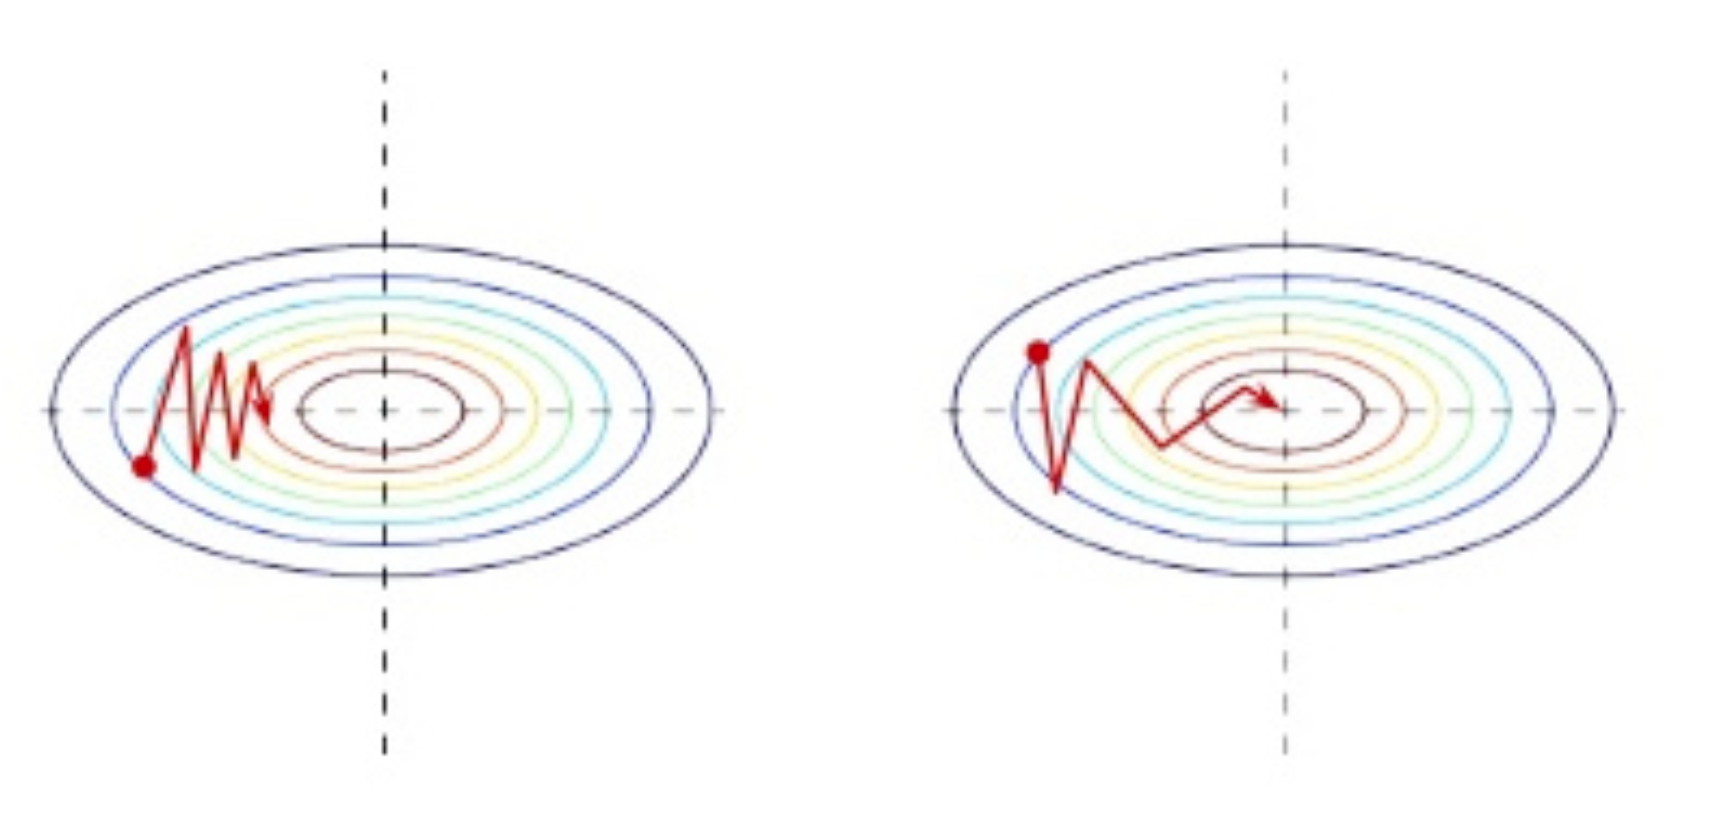
\includegraphics[width=0.5\linewidth]{img/sgd_mom.png}
    \caption{For momentum-based SGD, for any component where the gradient is heading in the intended direction, momentum is accumulated in that direction. In this example, note a horizontal acceleration towards the centre.}
    
\end{figure}
\end{definitionbox}

\begin{definitionbox}{SGD with Nesterov momentum}
Stochastic Gradient Descent (SGD) with Nesterov momentum is an optimisation technique that aims to accelerate SGD by taking into account the direction of the previous gradient step. It is described as follows:
\begin{itemize}
    \item The loss \( \mathcal{L} \) is computed as the average of the loss function \( \ell \) over all examples \( x_i \) in the mini-batch:
    \[ \mathcal{L} = \frac{1}{n} \sum_{i} \ell(h(x_i), y_i) \]
    \item The gradient of the loss with respect to the weights is:
    \[ \nabla_w \mathcal{L}(W) = \frac{1}{n} \sum_{i} \nabla_w \ell(h(x_i), y_i) \]
    \item The Nesterov momentum update is defined as:
    \[ Z_{t+1} = \beta Z_t + \nabla_w \mathcal{L}(W_t - \eta\beta Z_t) \]
    Note the lookahead step occurring in the loss function. Compare this to basic momentum given by:
    \[ Z_{t+1} = \beta Z_{t} + \nabla_w \mathcal{L}(W_t) \]
    Nesterov momentum involves calculating the decaying moving average of the gradients of projected positions in the search space rather than the actual positions themselves.


    \item The weight update formula is then:
    \[ W_{t+1} = W_t - \eta Z_{t+1} \]
\end{itemize}
Nesterov momentum improves upon standard momentum by refining the direction of the step not only with the current gradient but also by looking ahead at where the next step would take the optimisation process. This anticipatory update prevents us from going too fast and results in more responsive gradient steps.

Nesterov momentum involves:
\begin{enumerate}
    \item Making a step in the direction of the accumulated gradient.
    \item Measuring the gradient in this new point and correct the direction.
\end{enumerate}
This approach can significantly accelerate the convergence of SGD, especially in the context of high curvature, noisy gradients, or small mini-batches.
\begin{figure}[H]
    \centering
    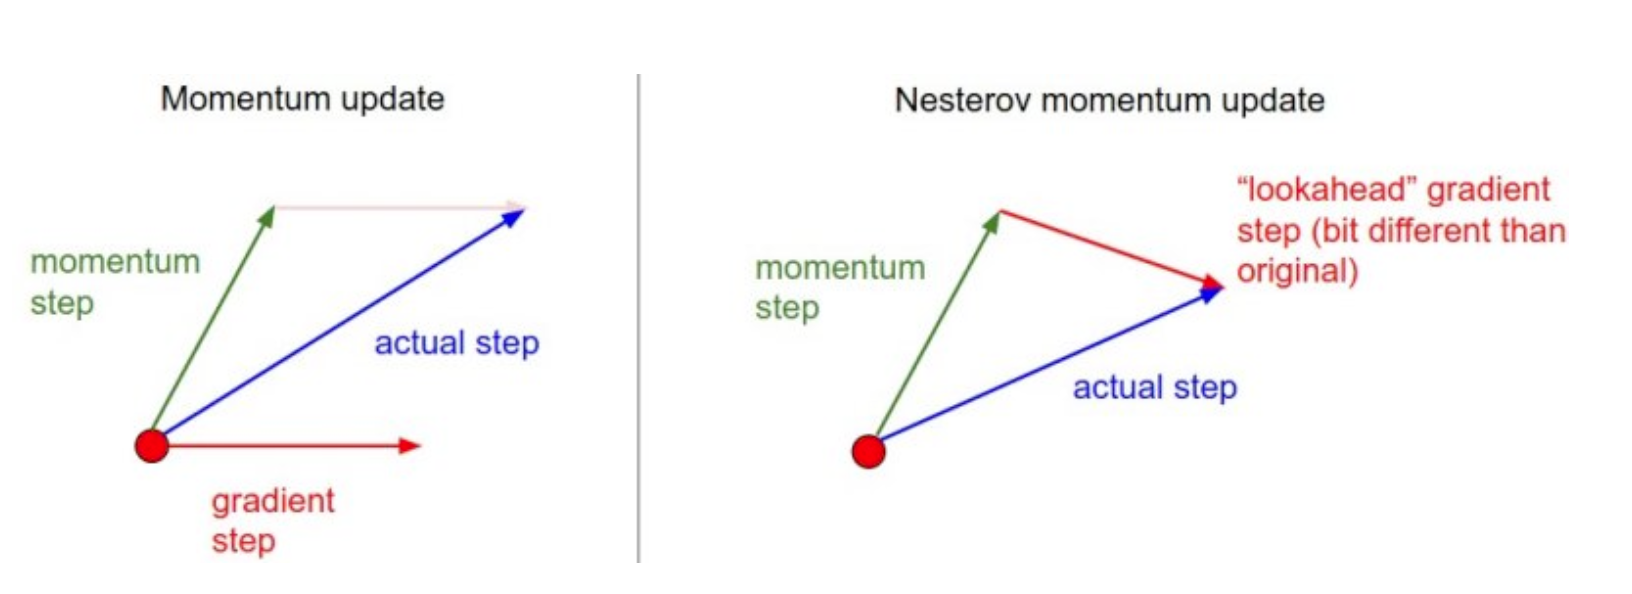
\includegraphics[width=0.7\linewidth]{img/nesterov.png}
    \caption{Lookahead gradient visualisation}
    
\end{figure}
\end{definitionbox}

\begin{definitionbox}{Adagrad}
Adagrad is an optimisation algorithm designed to adapt the learning rate to the parameters, performing smaller updates for parameters associated with frequently occurring features, and larger updates for parameters associated with infrequent features. It is particularly well-suited for dealing with sparse data. The Adagrad update rule is defined as follows:
\begin{itemize}
    \item The weight update rule is:
    \[ W_{t+1} = W_t - \frac{\eta}{\sqrt{G_t + \epsilon}} \odot \nabla_w \mathcal{L}(W_t) \]
    where \( G_t \in \mathbb{R}^{p \times p} \) is a diagonal matrix where each diagonal element \( i, i \) is the sum of the squares of the gradients with respect to \( w_i \) up to iteration \( t \), \( \eta \) is the learning rate, and \( \epsilon \) is a small smoothing term to prevent division by zero.
    \item Adagrad adapts the learning rate for each parameter, reducing the learning rate monotonically for each parameter.
    \item It has been used effectively in training GloVe word embeddings, among other applications.
    \item However, the monotonic decrease can sometimes lead to premature and excessive reduction in the effective learning rate, causing the algorithm to stop learning.
\end{itemize}

Intuitively, we are trying to step the weights vector through a (generally high) dimensional space trying to minimise the loss function. This is done by moving in the opposite direction to gradient. However, not all dimensions are equal. Some consistently receive larger gradients, some receive smaller gradients. If we use a uniform learning rate, we might step too far in directions with large gradients (potentially overshooting the minimum), and too little with small gradients (taking too long to converge). The diagonal matrix \(G\) is used to keep track of historical gradients, serving as an automatic tuning dial for learning rates.
\end{definitionbox}

\begin{definitionbox}{RMSProp}
RMSProp (Root Mean Square Propagation) is an adaptive learning rate method that adjusts the learning rate for each weight individually. It modifies the general gradient descent weight update rule as follows:
\begin{itemize}
    \item The weight update rule is:
    \[ W_{t+1} = W_t - \frac{\eta}{\sqrt{E[\nabla \mathcal{L}^2]_t + \epsilon}} \odot \nabla_w \mathcal{L}(W_t) \]
    \item The expected squared gradient \( E[\nabla \mathcal{L}^2]_t \) is the exponentially decaying average of squared gradients:
    \[ E[\nabla \mathcal{L}^2]_t = \gamma E[\nabla \mathcal{L}^2]_{t-1} + (1 - \gamma)(\nabla \mathcal{L}_t)^2 \]
\end{itemize}
Intuitively, RMSProp uses the magnitude of recent gradients to normalised the gradient; this is akin to adjusting the step size depending on the 'steepness' of the learning landscape. It prevents oscillations in directions with large gradients and allows for faster progress in directions with small gradients.
\end{definitionbox}

\begin{definitionbox}{Adadelta}
Adadelta is an extension of Adagrad that seeks to reduce its aggressive, monotonically decreasing learning rate. Instead of accumulating all past squared gradients, Adadelta limits the window of accumulated past gradients to some fixed size. The update rule is:
\begin{itemize}
    \item The weight update rule is:
    \[ W_{t+1} = W_t - \frac{\sqrt{E[\Delta W^2]_{t-1} + \epsilon}}{\sqrt{E[\nabla \mathcal{L}^2]_t + \epsilon}} \odot \nabla_w \mathcal{L}(W_t) \]
    \item The update accumulation \( E[\Delta W^2]_t \) is computed as:
    \[ E[\Delta W^2]_t = \gamma E[\Delta W^2]_{t-1} + (1 - \gamma)(W_t - W_{t-1})^2 \]
\end{itemize}
Intuitively, Adadelta adapts the learning rate based on a moving window of gradient updates, rather than accumulating all past squared gradients. This allows the learning rate to remain more robust and not decay to infinitesimally small values, which addresses the vanishing learning rate problem of Adagrad.
\end{definitionbox}

\begin{definitionbox}{Adam (Adaptive Moment Estimation)}
Adam is an optimisation algorithm that computes adaptive learning rates for each parameter by estimating the first and second moments of the gradients. Its update rule combines the advantages of two other extensions of stochastic gradient descent, AdaGrad and RMSProp. Specifically, the Adam update rule is given by:
\begin{itemize}
    \item The weight update rule is:
    \[ W_{t+1} = W_t - \frac{\eta}{\sqrt{v_t + \epsilon}} \odot m_t \]
    \item The first moment \( m_t \) and second moment \( v_t \) estimates are:
    \[ m_t = \frac{\beta_1 m_{t-1} + (1 - \beta_1) \nabla_w \mathcal{L}_t}{1 - \beta_1^t} = \frac{\mathbb{E}\left[ \nabla_w \mathcal{L}_t\right]}{1 - \beta_1^t} \]
    \[ v_t = \frac{\beta_2 v_{t-1} + (1 - \beta_2) (\nabla_w \mathcal{L}_t)^2}{1 - \beta_2^t} = \frac{\mathbb{E}\left[ \nabla_w \mathcal{L}_t\right]}{1 - \beta_1^t} \]
\end{itemize}
Intuitively, Adam performs smaller updates for parameters associated with frequently occurring features and larger updates for parameters associated with infrequent features. It uses the squared gradients to scale the learning rate and takes advantage of momentum by using the moving average of the gradient. It corrects for the initial bias towards zero in the first and second moment estimates, providing a more accurate update step.

Commonly used values for the decay parameters are \( \beta_1 \approx 0.9 \), \( \beta_2 \approx 0.999 \), and \( \epsilon \approx 10^{-8} \), which control the exponential decay rates for these moment estimates.
\end{definitionbox}

\subsection{Comparison of Optimisers}
\begin{figure}[H]
    \centering
    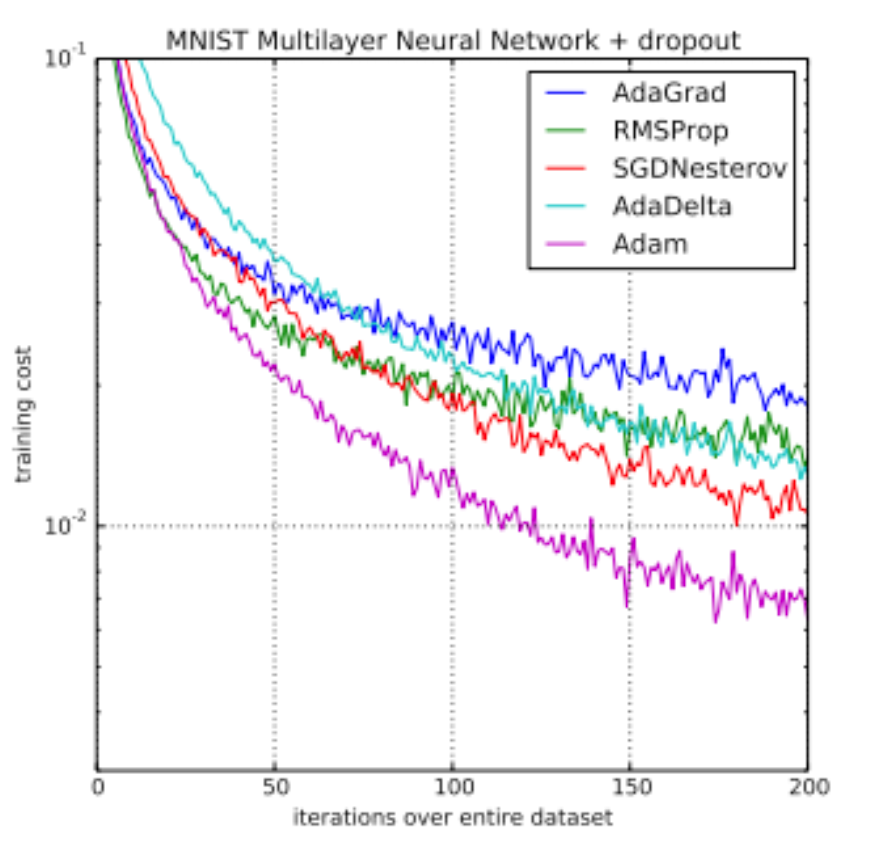
\includegraphics[width=0.5\linewidth]{img/optimisers.png}
    \caption{Comparison of training cost over iterations for different optimisers]}
    
\end{figure}

\begin{itemize}
    \item Adagrad introducing an adaptive learning rate, best suited for sparse data.
    \item RMSProp resolves vanishing learning rates by using decaying averages
    \item Adadelta is similar to RMSProp but does not require a learning rate
    \item Adam is RMSProp + Momentum, also adds bias correction
    \item SGD is often used, tends to find a good minimiser and generalises well
\end{itemize}

\section{Regularisation}
\subsection{Dropout}
Dropout is a regularisation technique for reducing overfitting in neural networks by preventing complex co-adaptations on training data. It is a very efficient way of performing model averaging with neural networks.

\begin{itemize}
    \item \textbf{Training Phase:}
    \begin{itemize}
        \item Randomly ignore (zero out) a fraction \( p \) of nodes (neurons) and their connections during each training iteration.
        \item This "thinning" of the network varies with each training sample, promoting feature robustness.
    \end{itemize}
    \item \textbf{Testing Phase:}
    \begin{itemize}
        \item Utilise all activations, but their outputs are scaled by \( p \) to balance the larger number of active nodes compared to the training phase.
    \end{itemize}
\end{itemize}

Dropout encourages the network to learn more robust features that are beneficial across various subsets of the other neurons, effectively reducing the risk of overfitting. For a layer with \( |W| \) nodes, there are \( 2^{|W|} \) possible subnetworks created by dropout, offering a rich ensemble of models for training. However, only one deterministic network is used for testing.

\begin{itemize}
    \item \textbf{Considerations:}
    \begin{itemize}
        \item Dropout can approximately double the number of iterations required to converge. Nevertheless, training time for each epoch might be reduced due to the simplified network.
        \item While dropout is effective for fully connected (FC) layers, it is less so for convolutional layers, which are less prone to overfitting due to their shared weights and locality constraints.
    \end{itemize}
\end{itemize}

\begin{figure}[H]
    \centering
    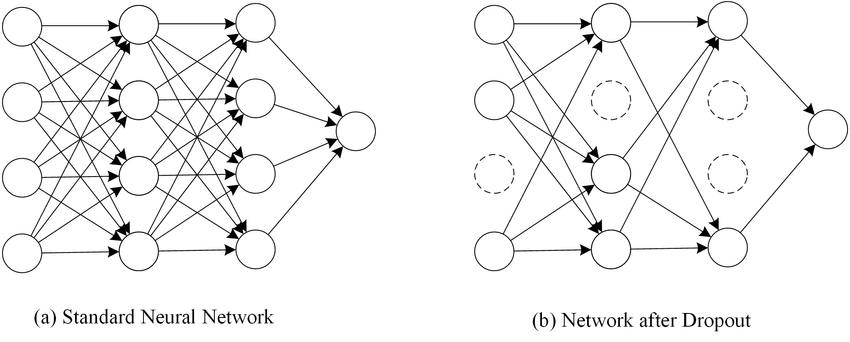
\includegraphics[width=0.75\linewidth]{img/dropout.png}
    
    \label{fig:dropout}
\end{figure}
\subsection{Distribution Problem}
Differences in the input distribution to neurons can lead to issues like saturation where the neuron's activation becomes less sensitive to changes in input.
\begin{itemize}
    \item During training, weights in early layers change and the inputs of later layers highly vary.
    \item Each layer has to readjust its weights to the varying distribution of every batch of inputs, which slows training.
    \item This varying input distribution also affects the neuron output, causing it to saturate its activation function. For extremely high or low values substituted into the activation function, its derivative at these regions are close to zero.
\end{itemize}

\begin{figure}[H]
    \centering
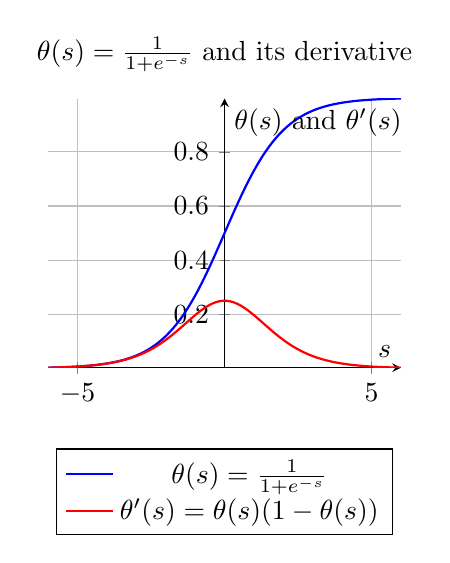
\begin{tikzpicture}
\begin{axis}[
    title={$\theta(s) = \frac{1}{1 + e^{-s}}$ and its derivative},
    axis lines=middle,
    width=0.5\textwidth,
    height=5cm,
    grid=major,
    domain=-6:6,
    legend style={at={(0.5,-0.3)},anchor=north},
    xlabel={$s$},
    ylabel={$\theta(s)$ and $\theta'(s)$},
    samples=100,
]
% sigmoid function
\addplot[blue, thick] {1/(1 + exp(-x))};
\addlegendentry{$\theta(s) = \frac{1}{1 + e^{-s}}$}

% derivative of the sigmoid function
\addplot[red, thick] {1/(1 + exp(-x))*(1 - 1/(1 + exp(-x)))};
\addlegendentry{$\theta'(s) = \theta(s)(1 - \theta(s))$}

\end{axis}
\end{tikzpicture}
\end{figure}

\begin{itemize}
    \item \textbf{Activation Analysis:}
    \begin{itemize}
        \item Monitoring the mean and standard deviation of activation values can reveal how activations evolve during training.
        \item The saturation of neurons in higher layers occurs rapidly if not properly normalised, causing the gradients to vanish during backpropagation.
    \end{itemize}
    \item \textbf{Histograms of Activation and Gradients:}
    \begin{itemize}
        \item These histograms can reveal changing patterns across layers, guiding the use of techniques like batch normalisation to maintain healthy distributions of activations.
    \end{itemize}
\end{itemize}

\begin{figure}[H]
    \centering
    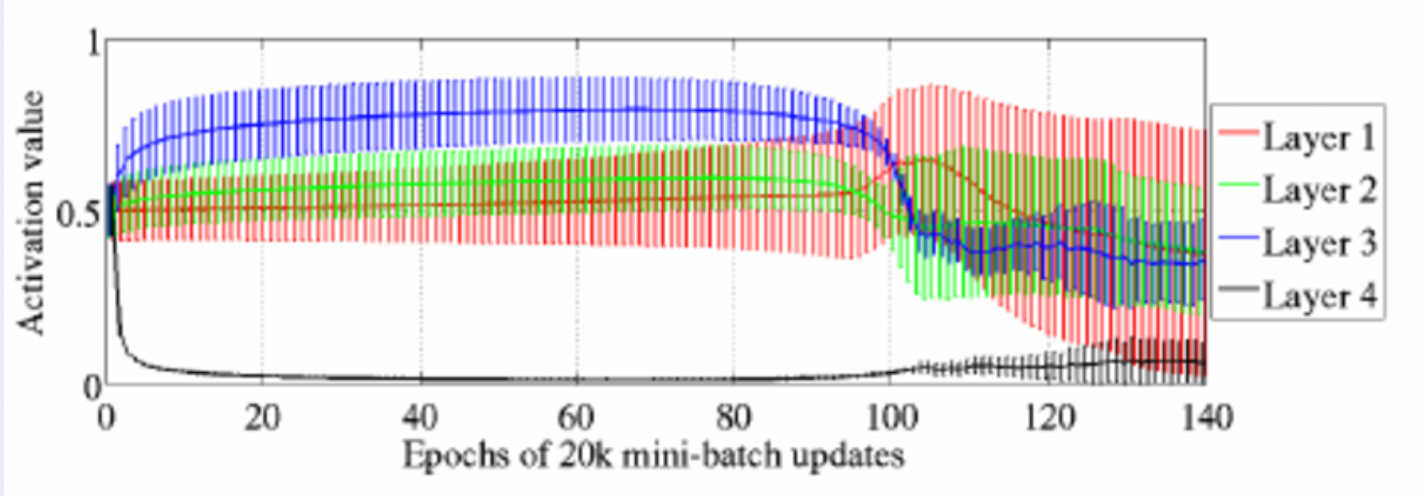
\includegraphics[width=0.75\linewidth]{img/distprob.png}
    \caption{Mean and standard deviation of activation values. Notice how they start to fluctuate after 100 epochs.}
    \label{fig:distprob}
\end{figure}

\begin{figure}[H]
    \centering
    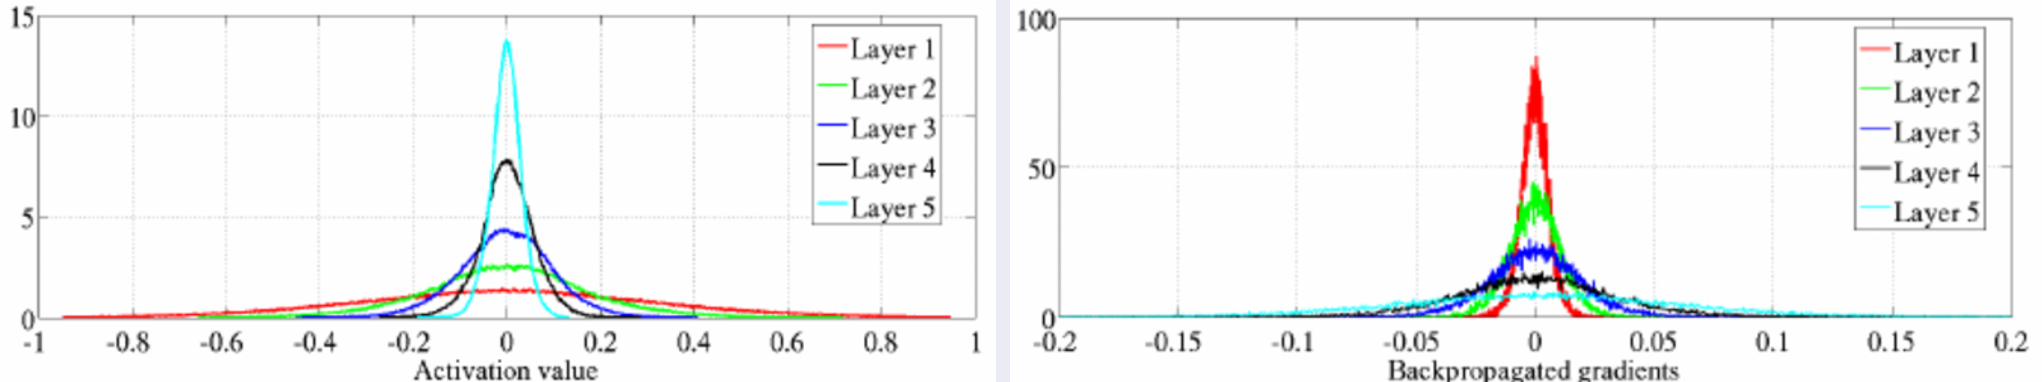
\includegraphics[width=0.75\linewidth]{img/activationgradienthistograms.png}
    \caption{Notice  higher activation levels correlate with smaller gradients—suggests that as the activations become more pronounced (potentially moving away from zero), the gradients diminish. }
    \label{fig:accgradhis}
\end{figure}

In Figure \ref{fig:accgradhis}, the distributions of the activation values at each layer suggest that the activations are relatively healthy, meaning they are not saturating to the extremes of the activation function (e.g., not all getting stuck at -1 or 1 for a tanh activation function).\\

The gradients' histograms show a clear decrease in their magnitude moving towards the earlier layers, from Layer 5 to 1. This is a sign of the vanishing gradients problem – as the gradient is backpropagated, the repeated multiplication can cause the gradient to become increasingly small. Consequently, the weights in the earlier layers (closer to the input) receive very small updates, which can significantly slow down the learning of these layers or stop it altogether. This is worsened in deep networks, when gradients have to propagate back through many layers, tending to decrease slightly each layer.

\subsection{Batch Normalisation}
The solution to the distribution problem is initialisation: normalising the weight distribution to ensure signal propagation. Proper weight initialisation is crucial to ensure effective signal propagation through the network during both the forward and backward passes. 

\subsubsection*{Assumptions for Initialisation}
\begin{itemize}
    \item The activation function is linear in the initial phase of training, \(\theta(s) = s\).
    \item The inputs to the network, \(x^{(0)}\), are assumed to have a zero mean and be independently and identically distributed (i.i.d.).
    \item The initial weight distribution for each layer is also i.i.d. with zero mean.
\end{itemize}

\subsubsection*{Variance Propagation}
To maintain the variance of the activations and backpropagated gradients throughout the layers, we aim for the following:

\begin{equation}
    \text{Var}[x^{(l)}] = \text{Var}[x^{(0)}] \prod_{k=1}^{l-1} d^{(k)} \text{Var}[W^{(k)}]
\end{equation}
\begin{equation}
    \text{Var}[\delta^{(l)}] = \text{Var}[\nabla \mathcal{L}] \prod_{k=l}^{L-1} d^{(k+1)} \text{Var}[W^{(k)}]
\end{equation}

where:
\begin{itemize}
    \item \(\text{Var}[x^{(k)}]\) and \(\text{Var}[W^{(k)}]\) represent the variance in the inputs and weight matrix at layer \(k\) respectively.
    \item \(\text{Var}[\delta^{(l)}]\) is the variance of the backpropagated error gradients.
    \item \(\nabla \mathcal{L}\) denotes the gradient of the cost function with respect to the activations.
    \item \(d^{(k)}\) denotes the number of neurons in layer \(k\).
\end{itemize}

\subsubsection*{Maintaining Variance Equilibrium}
To ensure that the signal does not vanish or explode as it propagates through the network, we require that the variance of the activations remains the same across each layer:

\begin{equation}
    \text{Var}[x^{(l)}] \approx \text{Var}[x^{(l+1)}] \Rightarrow d^{(l)} \text{Var}[W^{(l)}] = 1 \quad \forall l
\end{equation}

Similarly, for the backpropagated gradients:

\begin{equation}
    \text{Var}[\delta^{(l)}] \approx \text{Var}[\delta^{(l+1)}] \Rightarrow d^{(l+1)} \text{Var}[W^{(l)}] = 1 \quad \forall l
\end{equation}

\subsubsection*{The Symmetry Problem}
In general practice, biases can be safely initialised to zero since they do not contribute to the input of a neuron in the same way that weights do. However, weights require more initialisation to ensure proper learning.\\

When weights are initialised from a uniform or Gaussian distribution, it introduces asymmetry among the neurons, which allows them to learn different features. On the other hand, if all weights are initialised to zero, the neurons in each layer will perform the same computation, resulting in identical gradients during backpropagation. This means that:

\begin{equation}
    \frac{\partial \mathcal{L}}{\partial w_{ij}} = \frac{\partial \mathcal{L}}{\partial w_{ik}} \quad \forall j, k \quad \text{where} \quad w_{ij}, w_{ik} \in W^{(l)}
\end{equation}

Here, \(\mathcal{L}\) represents the loss function, and \(W^{(l)}\) represents the weight matrix at layer \(l\).\\

If this symmetry is not broken, it means that all neurons in a layer are learning the same features during training. This is known as the \emph{symmetry problem} and effectively makes the hidden units operate as if they are a single neuron. As a result, no matter how many neurons there are in a layer, it will be equivalent to having a single neuron—mirroring the capabilities of a linear model—thus severely limiting the capacity of the neural network to capture complex patterns.\\

To avoid this, initialise weights with small random values. The use of randomisation breaks the symmetry, allowing each neuron to learn different aspects of the input data and contribute to different parts of the output.

\subsubsection*{Xavier Initialisation for Sigmoid Activation}
For networks utilising sigmoid activation functions, Xavier (also called Glorot) initialisation is recommended:
\begin{itemize}
    \item Weights are initialised according to a variance that keeps the signal's variance constant through layers, which is given by:
    \begin{equation}
        \text{Var}[W^{(l)}] = \frac{2}{d^{(l)}+d^{(l+1)}}
    \end{equation}
    \item An example for weight initialisation:
    \begin{equation}
        W^{(l)} = U\left[-\frac{\sqrt{6}}{\sqrt{d^{(l)}+d^{(l+1)}}}, \frac{\sqrt{6}}{\sqrt{d^{(l)}+d^{(l+1)}}}\right], \quad b^{(l)} = 0
    \end{equation}
\end{itemize}
where \(d^{l}\) and \(d^{l+1}\) are the number of neurons in the previous and subsequent layers, respectively. This initialisation strategy ensures that the weights are neither too small nor too large, thus maintaining the signal's variance throughout the network, and is particularly effective for activation functions like the hyperbolic tangent.\\

\subsubsection*{Kaiming He Initialisation for ReLU Activations}
For networks with ReLU activations, Kaiming He initialisation is preferred:
\begin{itemize}
    \item The initialisation is adjusted to account for the rectifying nature of ReLU, which is typically inactive for half of its input, resulting in a variance that compensates for this:
    \begin{equation}
        \text{Var}[W^{(l)}] = \frac{2}{d^{(l)}}, \quad \text{for all layers } l \neq 1
    \end{equation}
    \item Special care is taken for the first layer since ReLU is not applied to the input signal:
    \begin{equation}
        \text{Var}[W^{(1)}] = \frac{1}{d^{(1)}}
    \end{equation}
\end{itemize}



\subsubsection*{Orthogonalisation}
Orthogonalisation is another technique to initialise weights, particularly useful for deep networks to mitigate the vanishing or exploding gradient problem.
\begin{itemize}
    \item This technique is informed by the desire to maintain the norm of the signal through layers, as seen in the propagation of gradients during backpropagation:
    \begin{equation}
        \delta^{(l)} = \left(\prod_{k=l}^{L-1} \theta'(s^{(k)})W^{(k)T}\right) \theta'(h(x))\nabla_{\!C}
    \end{equation}
    \item In practice, this is achieved by randomly initialising a weight matrix \(\widetilde{W}\) and then computing its singular value decomposition:
    \begin{equation}
        \widetilde{W} = U \Sigma V^T
    \end{equation}
    \item The matrix \(V^T\) (or \(U\) for non-square matrices) is then used as the initial weight matrix to ensure orthogonal weight vectors, which helps in preserving the magnitude of the forward and backward signals throughout the layers.
\end{itemize}



\begin{figure}[ht]
    \centering
    \begin{subfigure}[b]{0.5\textwidth}
        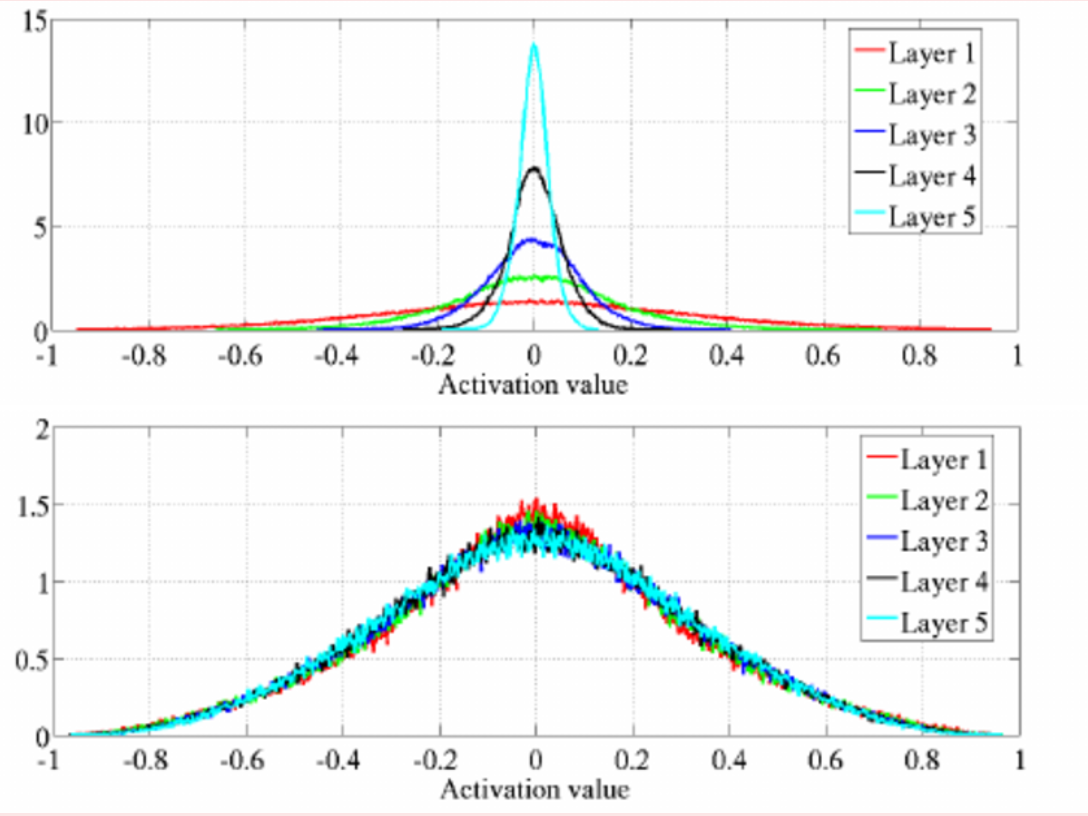
\includegraphics[width=\linewidth]{img/initcomparison1.png}
        \caption{Activation values}
        \label{fig:initcomp1}
    \end{subfigure}%
    \begin{subfigure}[b]{0.5\textwidth}
        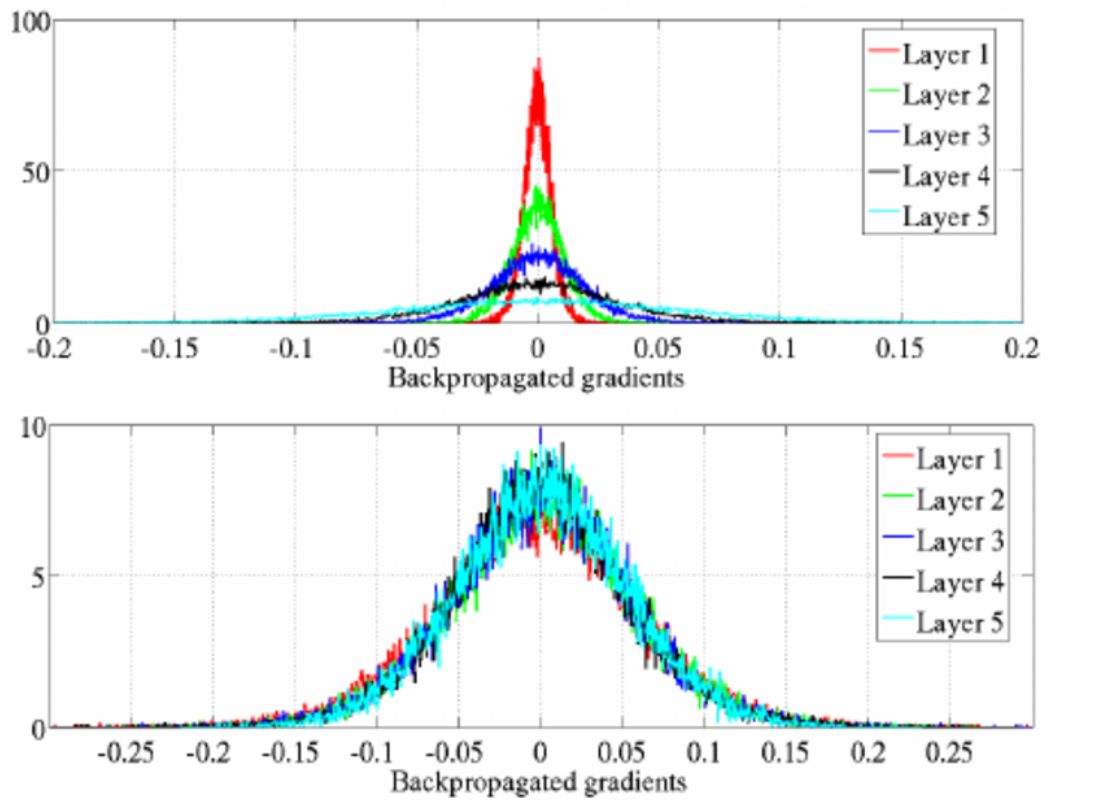
\includegraphics[width=\linewidth]{img/initcomparison2.png}
        \caption{Backpropagated gradients}
        \label{fig:initcomp2}
    \end{subfigure}
    \caption{Comparison between unnormalised initialisation and Xavier initialisation.}
    \label{fig:initcomparisons}
\end{figure}



\subsection{Revisiting Batch Normalisation}
\begin{figure}[H]
    \centering
    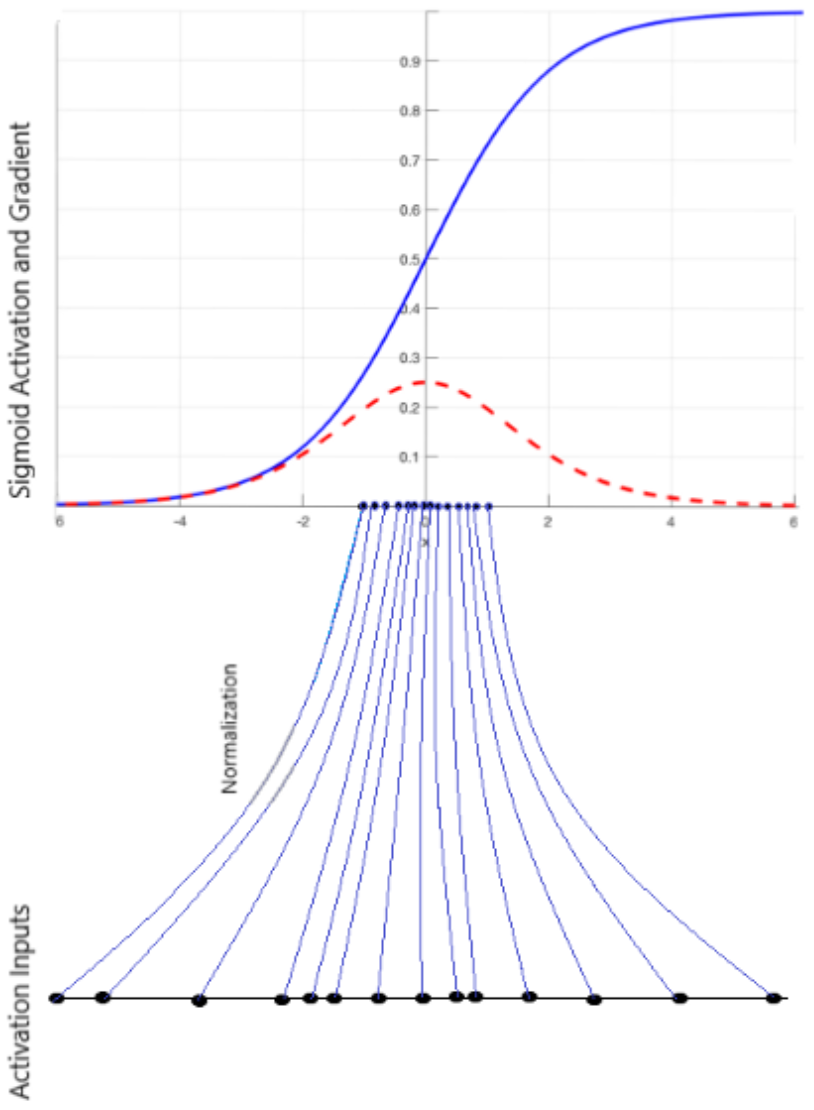
\includegraphics[width=0.4\linewidth]{img/sigmoid_bn.png}
     \caption{An illustration of the effect of Batch Normalisation on the activation values and gradients.}
\end{figure}

Batch Normalisation (BN) is a technique to accelerate the training of deep neural networks and improve their performance by stabilising the learning process.

\subsubsection*{Objectives and Benefits}
\begin{itemize}
    \item By normalising the inputs to each layer, Batch Normalisation allows the network to learn the distinguishing features between different classes more effectively.
    \item Constraining the neuron outputs to a 'sweet spot' of the activation function ensures the passage of substantial gradients during the backpropagation process. This typically results in:
    \begin{itemize}
        \item Shorter training times.
        \item Enhanced performance of the model.
    \end{itemize}
\end{itemize}

\subsubsection*{Training Phase}
During the training phase, Batch Normalisation performs the following transformations:
\begin{itemize}
    \item It normalises the layer outputs to a Gaussian distribution with zero mean and unit variance:
    \begin{equation}
        \hat{x} = \frac{x - \mu_B}{\sqrt{\sigma^2_B + \epsilon}}
    \end{equation}
    where \( \mu_B \) is the batch mean, \( \sigma^2_B \) is the batch variance, and \( \epsilon \) is a small constant is added to avoid dividing by zero.
    \item After normalisation, the outputs are scaled and shifted by learned parameters \( \gamma \) and \( \beta \), which allow the network to undo the normalisation if that is beneficial for the model:
    \begin{equation}
        y = \gamma \hat{x} + \beta = BN_{\gamma,\beta}(\hat{x})
    \end{equation}
\end{itemize}

\subsubsection*{Testing Phase}
In the testing phase, Batch Normalisation uses the population statistics gathered during training instead of the batch statistics:
\begin{itemize}
    \item The normalisation is done using the mean and variance of the entire training population, which are calculated as averages of the respective batch means and variances computed during the training.
\end{itemize}

\subsubsection*{Overall Impact}
The integration of Batch Normalisation has a few important consequences:
\begin{itemize}
    \item It ensures that the inputs to each layer across different mini-batches are less variable, leading to more stable convergence patterns.
    \item \textbf{By placing the Batch Normalisation layer between the convolutional and activation layers}, it assists in maintaining a healthy gradient flow through the network, which can prevent the gradients from vanishing or exploding, particularly in deep networks.
\end{itemize}
\subsubsection*{Effect of Batch Normalisation}
\begin{figure}[H]
    \centering
    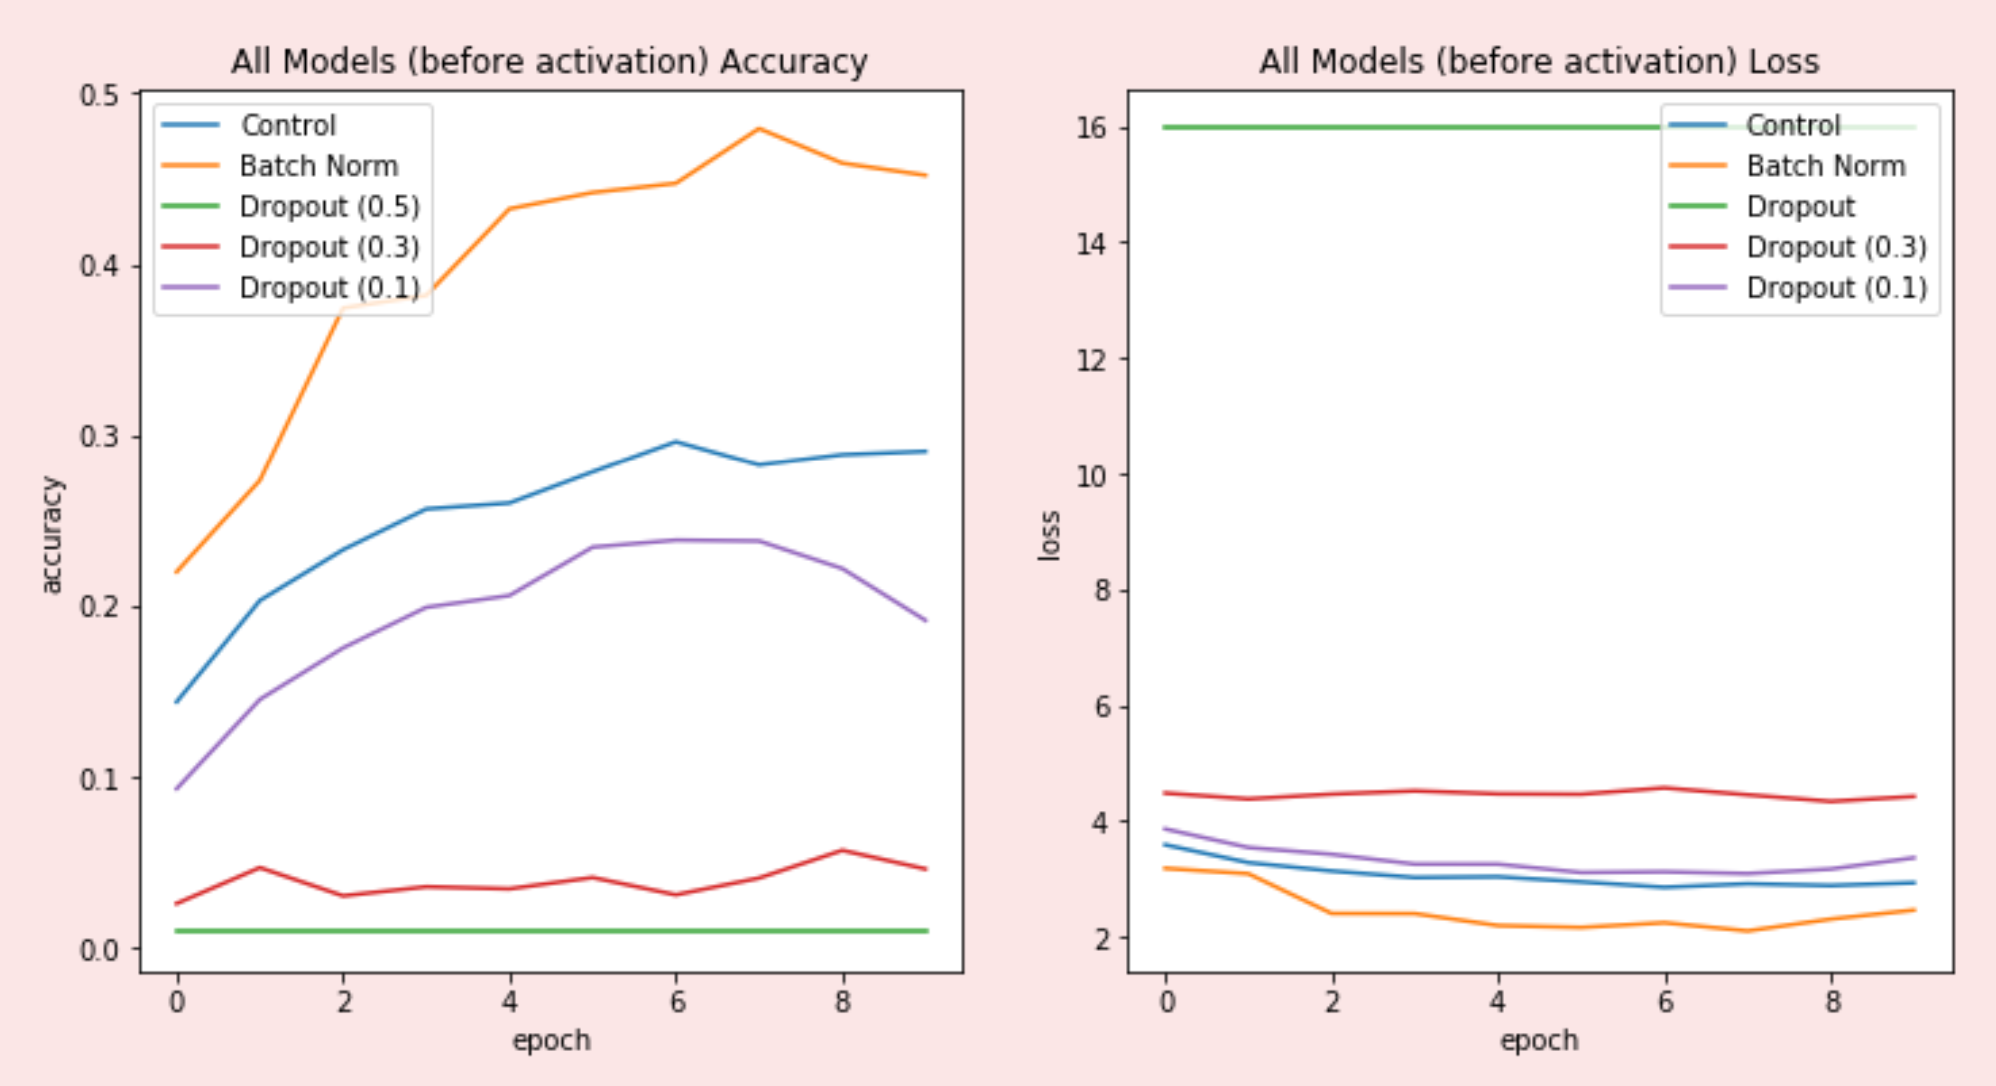
\includegraphics[width=0.65\linewidth]{img/bneffect.png}
    \caption{Note increased accuracy and lower loss over epochs}
\end{figure}


\subsubsection*{Advantages of Batch Normalisation}
\begin{itemize}
    \item \textbf{Approximation Through Mini-batches:} It would be ideal to whiten each layer's activation, but this is too computationally expensive. Batch Normalisation normalises each feature independently in each layer, utilising the mini-batch statistics to approximate the overall statistics of the training set.
    \item \textbf{Prevention of Vanishing Gradients:} It is particularly beneficial for networks with saturable nonlinearities, such as sigmoid or hyperbolic tangent activations, as it prevents the gradient from vanishing too quickly.
    \item \textbf{Regularisation:} Batch Normalisation also has a regularising effect, which can reduce the need for other regularisation techniques like dropout.
    \item \textbf{Training Efficiency:} It permits the use of higher learning rates, accelerating the training process and decreasing the time required to train the model.
    \item \textbf{Performance Improvement:} By maintaining the stability of the learning process, it often leads to better overall model performance.
    \item \textbf{Hyperparameter Tuning:} Batch Normalisation introduces additional hyperparameters that can be fine-tuned to further enhance model training.
\end{itemize}

\subsection{Batch Normalisation in Convolutional Networks}
In Convolutional Neural Networks (ConvNets), batch normalisation takes a slightly different approach:

\subsubsection*{Feature Map Normalisation}
\begin{itemize}
    \item Consider an input with shape \([N, H, W, C]\) where \(N\) is the number of examples in the mini-batch, \(H \times W\) are the dimensions of the feature map, and \(C\) is the number of channels.
    \item Traditional Batch Normalisation would calculate the mean and standard deviation across \(H \times W \times C\) to normalise each feature separately at each spatial location.
    \item In ConvNets, Batch Normalisation is adapted to compute the means and standard deviations across \(C\) and normalises jointly for all spatial locations.
    \item This approach respects the spatial structure of the input data, ensuring that the normalisation process considers the spatial patterns present within each feature map.
    \item Applying Batch Normalisation in ConvNets can lead to more detailed feature representations, as the normalisation across feature maps takes into account the spatial correlations, preserving important structural information.
\end{itemize}

\begin{figure}[ht]
\centering
\begin{subfigure}[b]{0.5\textwidth}
    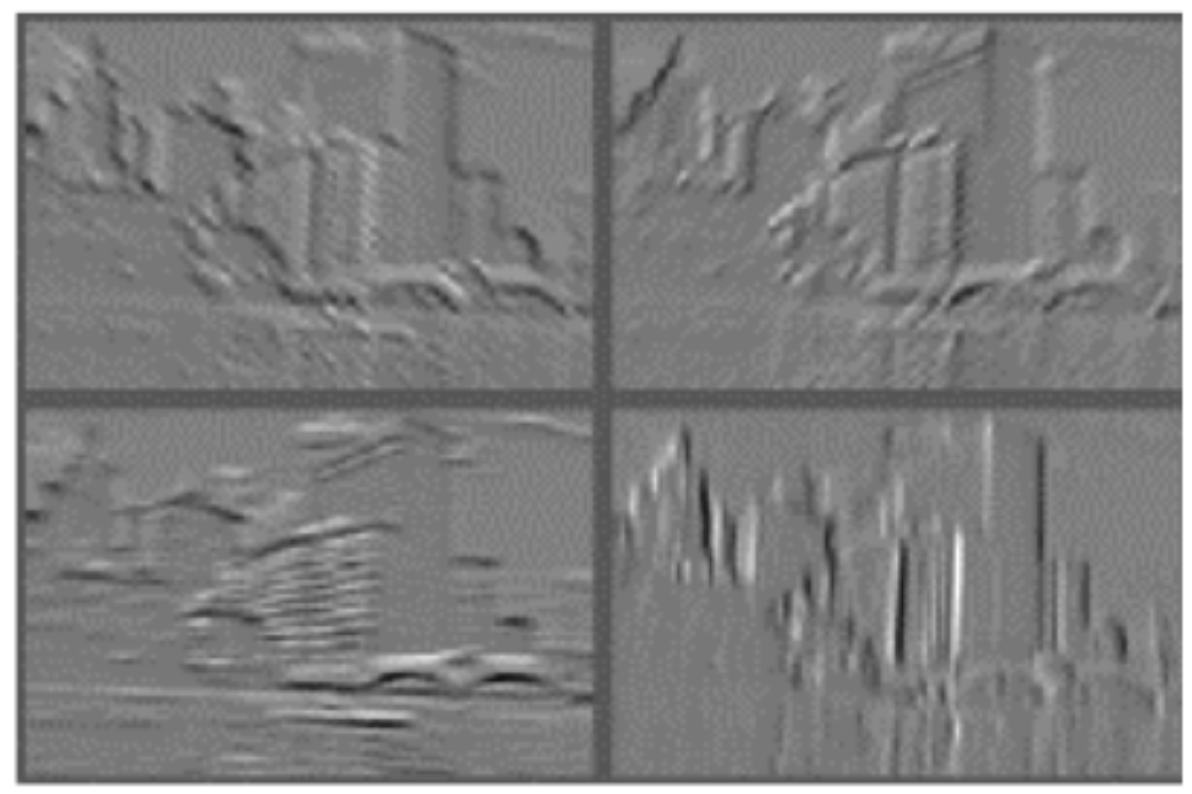
\includegraphics[width=\linewidth]{img/accmapNoBN.png}
    \caption{Activation map without BN}
\end{subfigure}%
\begin{subfigure}[b]{0.5\textwidth}
    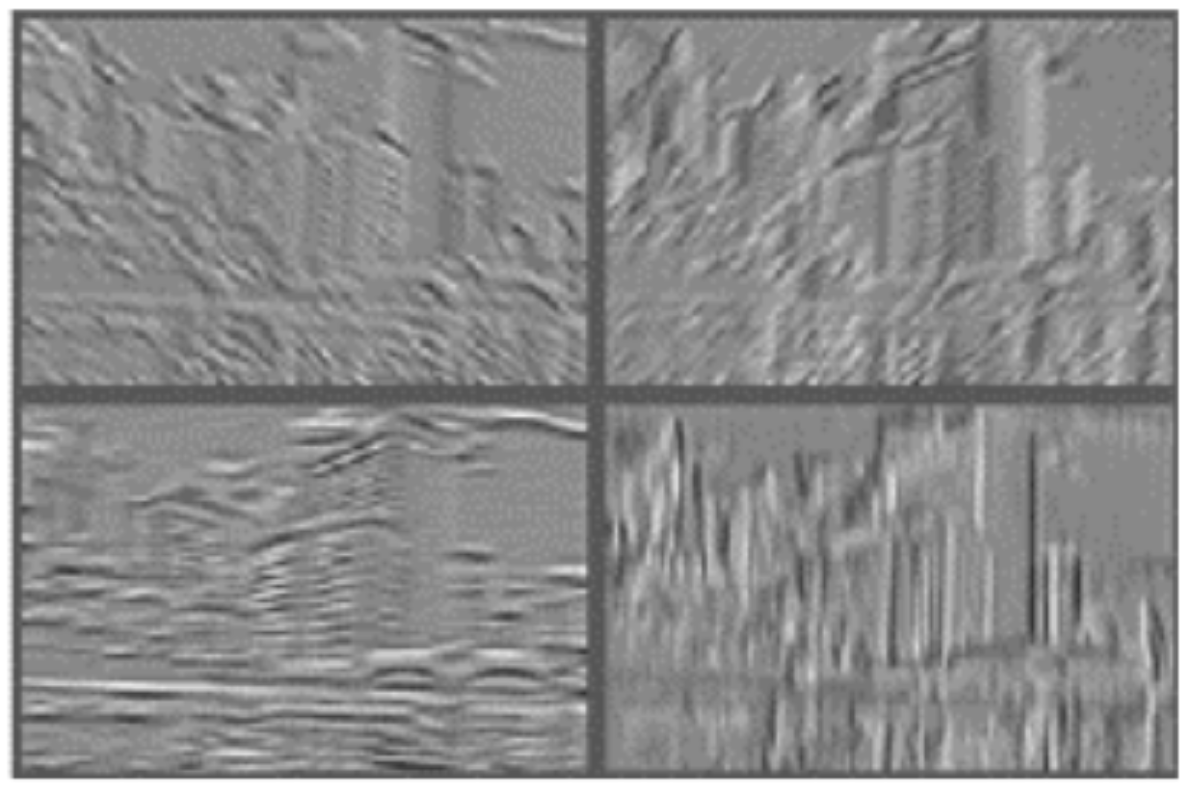
\includegraphics[width=\linewidth]{img/accmapBN.png}
    \caption{Activation map with BN}
\end{subfigure}
\caption{Comparison between details captured with or without BN in ConvNets}
\label{fig:accMapCompare}
\end{figure}


\section{Network Design and Finetuning}

\begin{figure}[H]
    \centering
    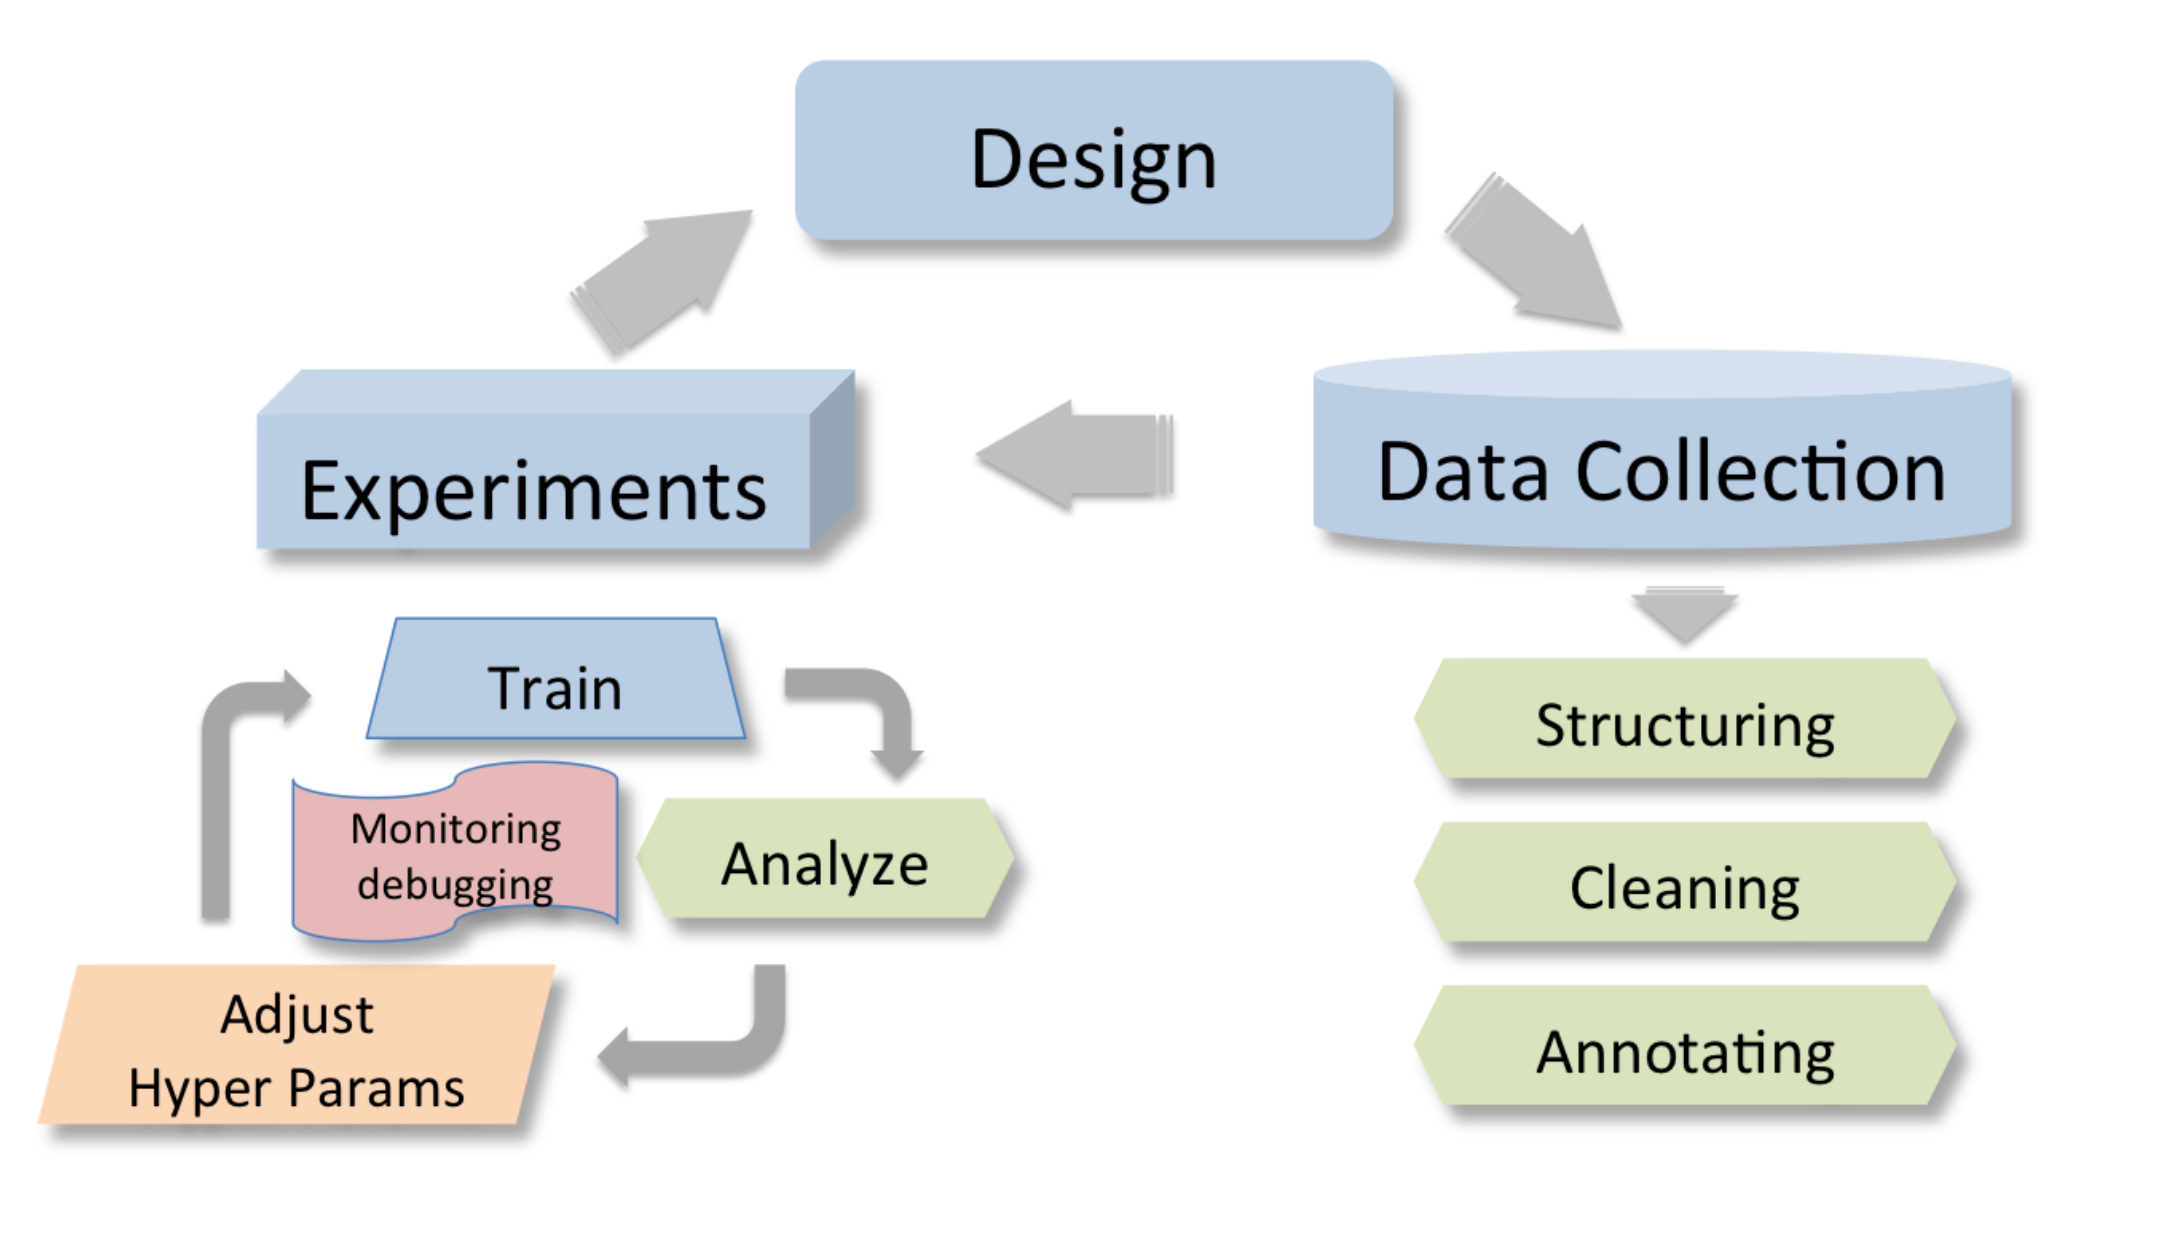
\includegraphics[width=0.75\linewidth]{img/desProcess.png}
    \caption{Flowchart visualisation of the development process}
\end{figure}
\subsection{Baseline Model}
It is important as a first step to establish a baseline model.

\subsubsection*{Literature Review}

 Prior to model construction, investigate whether the task has been addressed previously and conduct a comprehensive literature review. This can include analysing results from relevant competitions and survey papers to establish a credible end-to-end system.

\subsubsection*{Model Selection}

 Select an appropriate model based on the structure and nature of your data:
    \begin{itemize}
        \item Utilise Multilayer Perceptrons (MLP) for fixed-size vector inputs.
        \item Employ Convolutional Neural Networks (CNN) for image data.
        \item Choose Recurrent Neural Networks (RNN) for sequential or time-series data.
    \end{itemize}


\subsubsection*{Activation Functions}

Prefer non-linear activation functions that avoid the vanishing gradient problem:
    \begin{itemize}
        \item Refrain from using the sigmoid function except for the output layer in binary classification tasks.
        \item Use the Rectified Linear Unit (ReLU) activation function for hidden layers, but consider the Leaky ReLU variant to prevent dying ReLU problems, where neurons stop learning completely.
        \item Implement Maxout activations if a significant number of ReLU units are not active (dying).
    \end{itemize}


\subsubsection*{Weights and Biases Initialisation}
\begin{itemize}
    \item Initialise weights randomly with proper variance to break symmetry for efficient learning.
    \item For ReLU activations, a small positive bias can be advantageous to ensure that neurons initially activate and avoid the dying ReLU issue.
\end{itemize}

\subsection{Finetuning Strategy: Borrowing Knowledge}

Finetuning is an effective strategy for transferring knowledge from one domain to another, enhancing the learning process when starting from a pre-existing neural network.

\subsubsection*{Pretraining}

 Pretrain your neural network on a large dataset, which could be related in domain or task, or utilise a pretrained neural network as the starting point.


\subsubsection*{Adaptation Methods}

To adapt the pretrained network to a new task, you have two primary options:
\begin{itemize}
    \item Modify the architecture by removing or reshaping the last few layers and using the features extracted from earlier layers.
    \item Finetune the model parameters using your own dataset.
        \item Freeze the parameters of the first few layers, or alternatively, set a smaller learning rate for these layers to retain most of the previously learned features.
        \item Depending on the size of your dataset:
        \begin{itemize}
            \item For small datasets, train only the last fully connected (FC) layers.
            \item For medium-sized datasets, other layers can also be finetuned.
        \end{itemize}
        \item Apply a reduced learning rate, such as 1/10th of the original learning rate for the top layer, and an even smaller rate, such as 1/100th, for intermediate layers.

\end{itemize}


\begin{figure}[H]
    \centering
    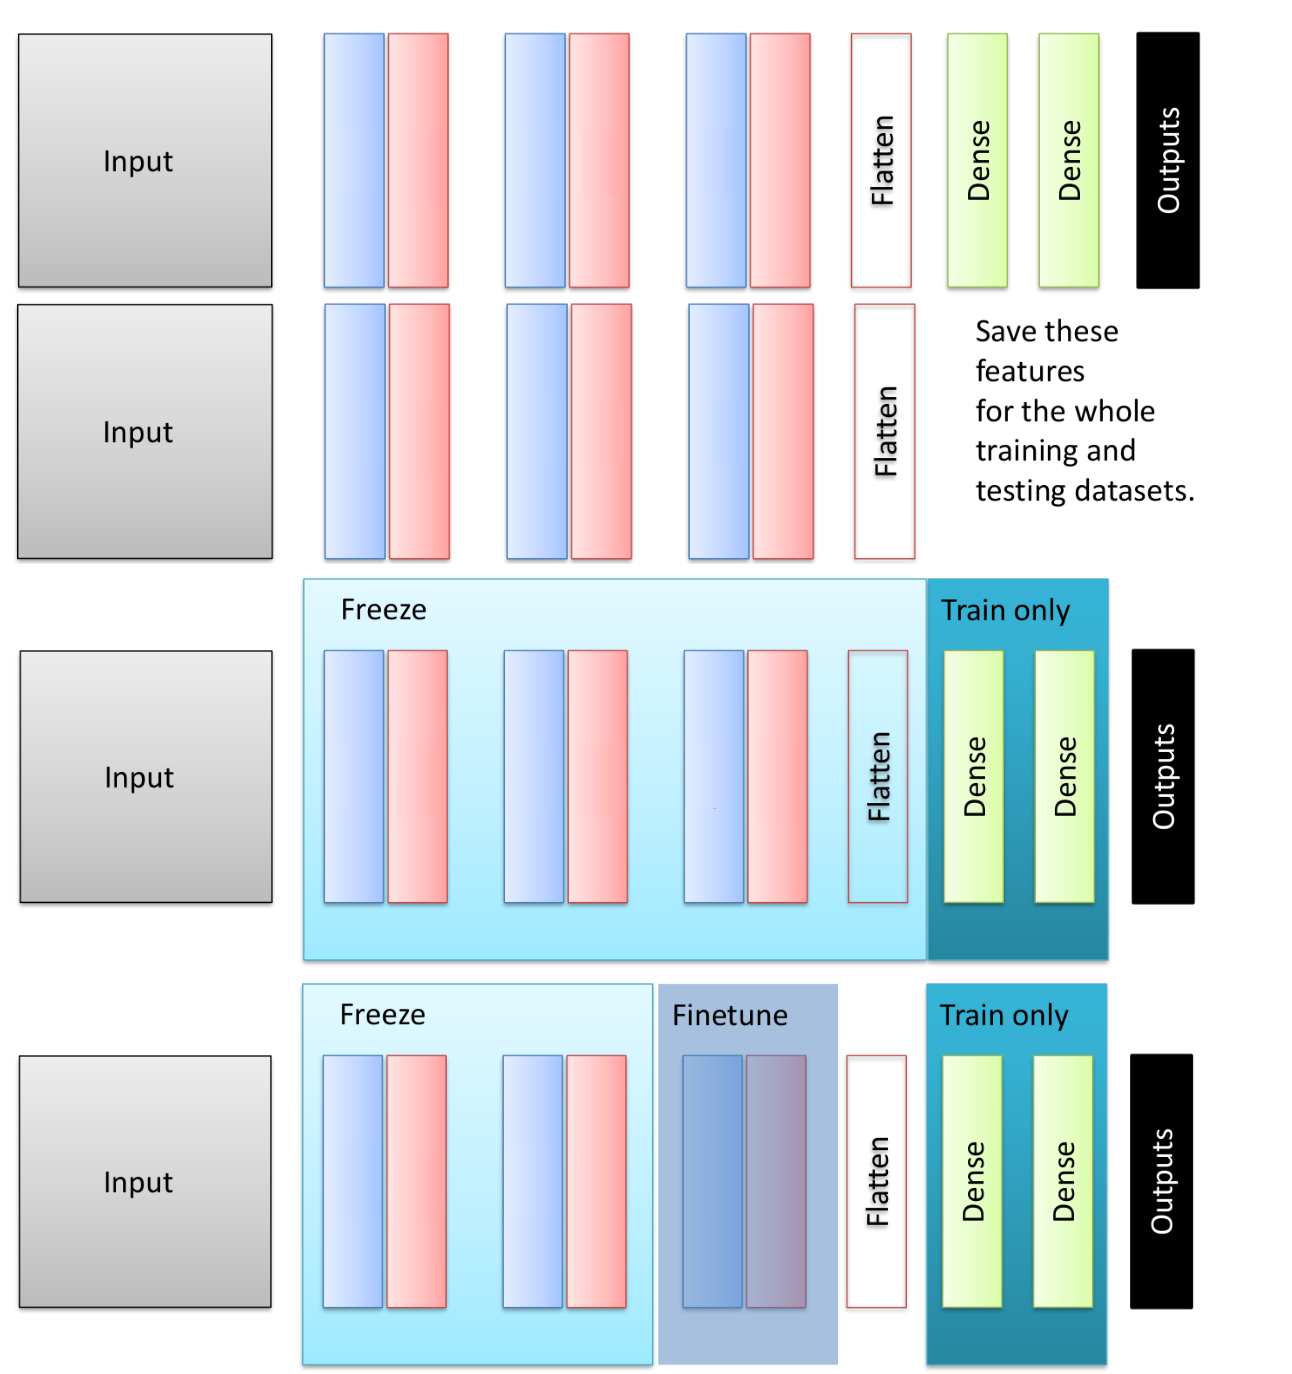
\includegraphics[width=0.7\linewidth]{img/finetune_freeze.png}
    \caption{Finetuning process visualised}
    
\end{figure}
\subsection{Data Collection}

The process of data collection is a foundational step in the development of machine learning models.

\subsubsection*{Quantity and Quality of Data}
\begin{itemize}
    \item The volume of data collected should be sufficient to capture the complexity of the problem. More data typically leads to more accurate models, but the quantity must be balanced against the cost of collection and diminishing returns.
    \item The required accuracy and the error bounds of the model should guide the amount of data needed.
\end{itemize}

\subsubsection*{Data Labelling}
\begin{itemize}
    \item Data labelling can be conducted using platforms such as Amazon Mechanical Turk, engaging freelancers, or consulting with domain experts to ensure high-quality annotations.
\end{itemize}

\subsubsection*{Bias Mitigation}
\begin{itemize}
    \item Avoiding bias in data collection is essential. Biases can arise from unrepresentative sampling or selective data collection practices. Strive for a dataset that accurately reflects the diversity of the real-world scenario.
\end{itemize}

\subsection{Dataset Preparation and Curation}

Once data is collected, it must be properly prepared and curated before it can be effectively used to train a machine learning model.

\subsubsection*{Structuring and Formatting}
\begin{itemize}
    \item Evaluate whether the format of the data is suitable for the task at hand, and conduct any necessary transformations to standardise the dataset.
\end{itemize}

\subsubsection*{Cleaning}
\begin{itemize}
    \item Cleaning the dataset involves addressing issues such as incomplete data, anonymisation requirements, missing annotations, and correcting errors in the dataset.
\end{itemize}

\subsubsection*{Normalisation}
\begin{itemize}
    \item Normalise the data by clipping extreme values and scaling features to a standard range. 
    \item Whitening, or decorrelation, is a technique to transform the input variables into a new space where they are uncorrelated and have the same variance.
\end{itemize}

\subsection{Data Splitting}

\subsubsection*{Training Set}
\begin{itemize}
    \item Typically comprises around \textbf{60\%} of the data and is used to train the model. 
    \item Essential to ensure that this data is balanced across different classes or outcomes to prevent training bias.
\end{itemize}

\subsubsection*{Validation Set}
\begin{itemize}
    \item Often \textbf{20\% o}f the data.
    \item The validation set is used to tune hyperparameters, select features, and make decisions regarding the learning algorithm without overfitting to the test set. 
    \item It is also referred to as the development set.
\end{itemize}

\subsubsection*{Test Set}
\begin{itemize}
    \item The test set also generally consists of\textbf{ 20\% }of the data.
    \item It is used to evaluate the performance of the algorithm after the learning process is complete.
\end{itemize}

\subsubsection*{Testing Phase}
\begin{itemize}
    \item Do not to use the test set to make decisions that might improve learning, as this can lead to overfitting and an overestimation of the model's performance on unseen data.
\end{itemize}


\subsection{Model Validation and Regularisation}

Validation is needed for assessing the performance of a hypothesis \( h \) or model \( g \) on a given machine learning task, by estimating \( \mathcal{L}_n (h) \).\\

Regularisation incorporates an overfit penalty to the loss function to avoid overfitting and enhance the model's ability to generalise. The regularised loss function is denoted as:

\begin{equation}
    \mathcal{L}_n (h) = \hat{R}_n (h) + \lambda \underbrace{\Omega(h)}_{\text{overfit penalty}}
\end{equation}



where:
\begin{itemize}
    \item \( \mathcal{L}_n (h) \) is the regularised loss.
    \item \( \hat{R}_n (h) \) represents the empirical risk.
    \item \( \lambda \) is the regularisation coefficient.
    \item \( \Omega(h) \) quantifies the complexity of the hypothesis \( h \).
\end{itemize}

\subsection{Validation Procedure}
The validation procedure involves several critical steps:
\begin{enumerate}
    \item The dataset \( \mathcal{D} \) is split into a training set \( \mathcal{D}_{\text{train}} \) and a validation set \( \mathcal{D}_{\text{val}} \).
    \item The model \( g \) is trained on \( \mathcal{D}_{\text{train}} \).
    \item The model's performance is estimated on \( \mathcal{D}_{\text{val}} \) using the equation:
    \begin{equation}
        \check{R}_{\text{val}} (g) = \frac{1}{v} \sum_{(x_i,y_i) \in \mathcal{D}_{\text{val}}} \ell(g(x_i), y_i)
    \end{equation}
    where \( v \) is the number of examples in the validation set, and \( \ell \) is the loss function.
\end{enumerate}
\begin{equation}
    \underbrace{\mathbb{E}_{\mathcal{D}_{{val}}}\left[\check{R}_{{v}}(g)\right]\approx R(g)}_{\text{very good estimate for }R(g)}\leqslant\ \check{R}_{\mathbf{v}}(g)+ \underbrace{\Omega(\mathbf{v},\mathbf{\delta})}_{\text{one model only on v-points} \sim \sqrt{\log (1/\delta)}} \quad \quad \text{with probability } 1-\delta
\end{equation}

This estimated performance \( \check{R}_{\text{val}} (g) \) is a good indicator of the true risk \( R(g) \) with high probability \( (1 - \delta) \) and $\mathcal{D}_{val}$ is a small, unbiased Hoeffding bound where only one $g$ (model) is considered. 

\subsection*{Regularisation and Model Selection}
The validation set \( \mathcal{D}_{\text{val}} \) is unbiased and can be used to select the optimal regularisation coefficient \( \lambda^* \) through the minimisation process:
    \begin{equation}
        \lambda^* = \underset{\lambda}{\text{argmin}} \, \check{R}_{\text{val}}(g)
    \end{equation}
After determining \( \lambda^* \), the final model can be trained on the entire dataset \( \mathcal{D} \) with \( \lambda^* \).



\subsection{Data Augmentation}
\subsubsection{Image Data Augmentation}
Data augmentation in the domain of images can significantly increase the diversity of data available for training models without actually collecting new data.

\begin{itemize}
    \item \textbf{Noise Addition:}
    \begin{itemize}
        \item Introduce variability through adding random noise to image pixels.
    \end{itemize}
    
    \item \textbf{Generating Modified Samples:}
    \begin{itemize}
        \item Create variations of the training samples to represent different possible scenarios.
    \end{itemize}
    
    \item \textbf{Medical Data:}
    \begin{itemize}
        \item Segmenting tumour masses to focus on regions of interest.
        \item Moving or rotating the segmented tumour to simulate different angles.
        \item Resampling background tissue to generalise over different textures.
        \item Blending images for realistic composites.
    \end{itemize}
\end{itemize}

\subsubsection{Text Data Augmentation}
Augmentation in text data involves modifications at the character or word level to create textual diversity.

\begin{figure}[H]
    \centering
    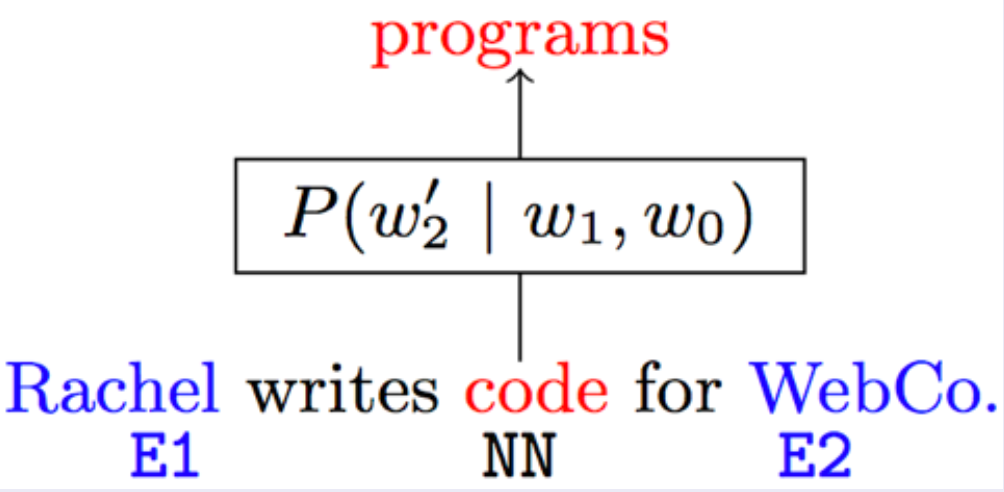
\includegraphics[width=0.5\linewidth]{img/text_aug.png}
    
    
\end{figure}

\begin{itemize}
    \item \textbf{Noise Addition:}
    \begin{itemize}
        \item Injecting typos or character-level noise to simulate common errors in text input.
    \end{itemize}
    
    \item \textbf{Synonym Insertion:}
    \begin{itemize}
        \item Substituting words with their synonyms to change the text while preserving meaning.
    \end{itemize}
    
    \item \textbf{Word Swap:}
    \begin{itemize}
        \item Using an external language model to perform conditional word swaps, targeting nouns or key entities in a sentence.
    \end{itemize}
    
    \item \textbf{Rare Words:}
    \begin{itemize}
        \item Including rare words in new contexts to improve the model's ability to understand and use them.
    \end{itemize}
\end{itemize}

\subsubsection{Audio Data Augmentation}
In the audio domain, augmentation can help a model become robust to various distortions and noise that occur in real-world scenarios.
\begin{figure}[H]
    \centering
    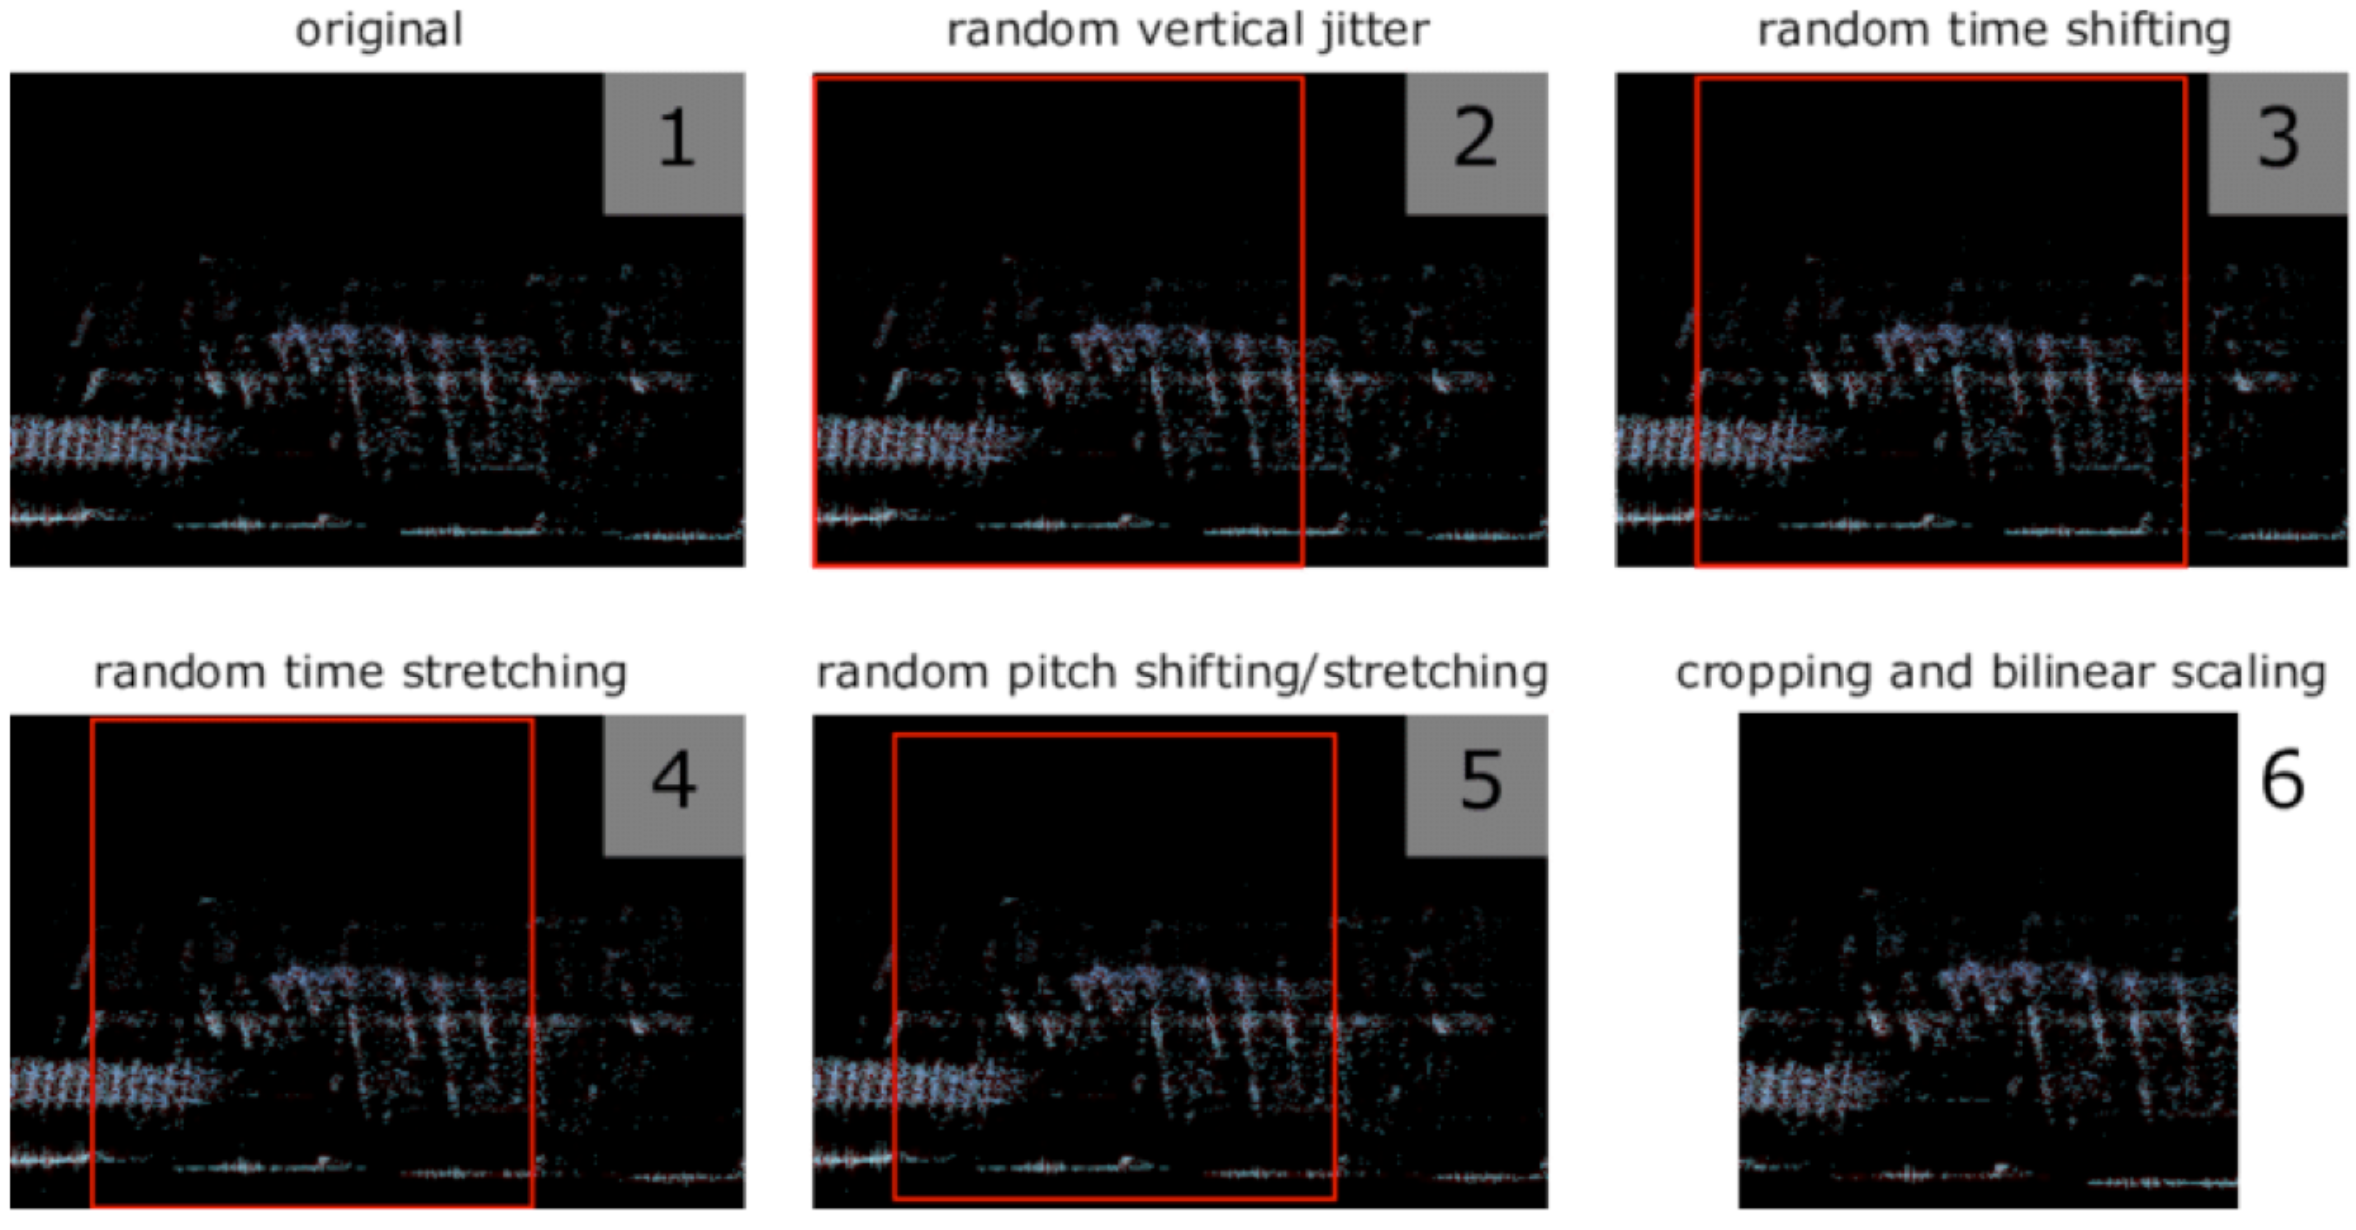
\includegraphics[width=0.8\linewidth]{img/audio_aug.png}
    
    
\end{figure}
\begin{itemize}
    \item \textbf{Adding Background Noise:}
    \begin{itemize}
        \item Incorporate different types of noise to mimic real-life auditory disturbances.
    \end{itemize}
    
    \item \textbf{Jitter:}
    \begin{itemize}
        \item Apply small, random shifts in the audio waveform to introduce robustness.
    \end{itemize}
    
    \item \textbf{Time-Based Transformations:}
    \begin{itemize}
        \item Shifting: Delay the audio signal to simulate temporal variations.
        \item Stretching: Alter the speed without changing the pitch to simulate faster or slower speech.
    \end{itemize}
    
    \item \textbf{Pitch Shifting:}
    \begin{itemize}
        \item Change the pitch of the audio signal to simulate different tonal variations.
    \end{itemize}
    
    \item \textbf{Cropping and Scaling:}
    \begin{itemize}
        \item Trim or scale audio waveforms to create samples of varying lengths and resolutions.
    \end{itemize}
\end{itemize}

\subsection{Adversarial Training (Hard Positive/Negative Mining)}
A technique to improve model robustness by focusing on challenging examples which are close to the decision boundary.


\begin{itemize}
    \item Form mini-batches with a balanced mix of hard positive and negative examples.
    \item Identify difficult examples during validation that are close to the decision boundary.
    \item Reintroduce these hard examples in subsequent training iterations to improve model discrimination.
\end{itemize}


Training models using examples that are specifically designed to be difficult for the model to classify.

\begin{definitionbox}{Hard Positive and Negative Examples}
\textbf{Hard Negatives} are examples incorrectly classified as positive, near the decision boundary.

\textbf{Hard Positives} are examples incorrectly classified as negative, near the decision boundary. 
    
\end{definitionbox}




\subsubsection*{Identity-Level Structure and Random Selection}
\begin{figure}[H]
    \centering
    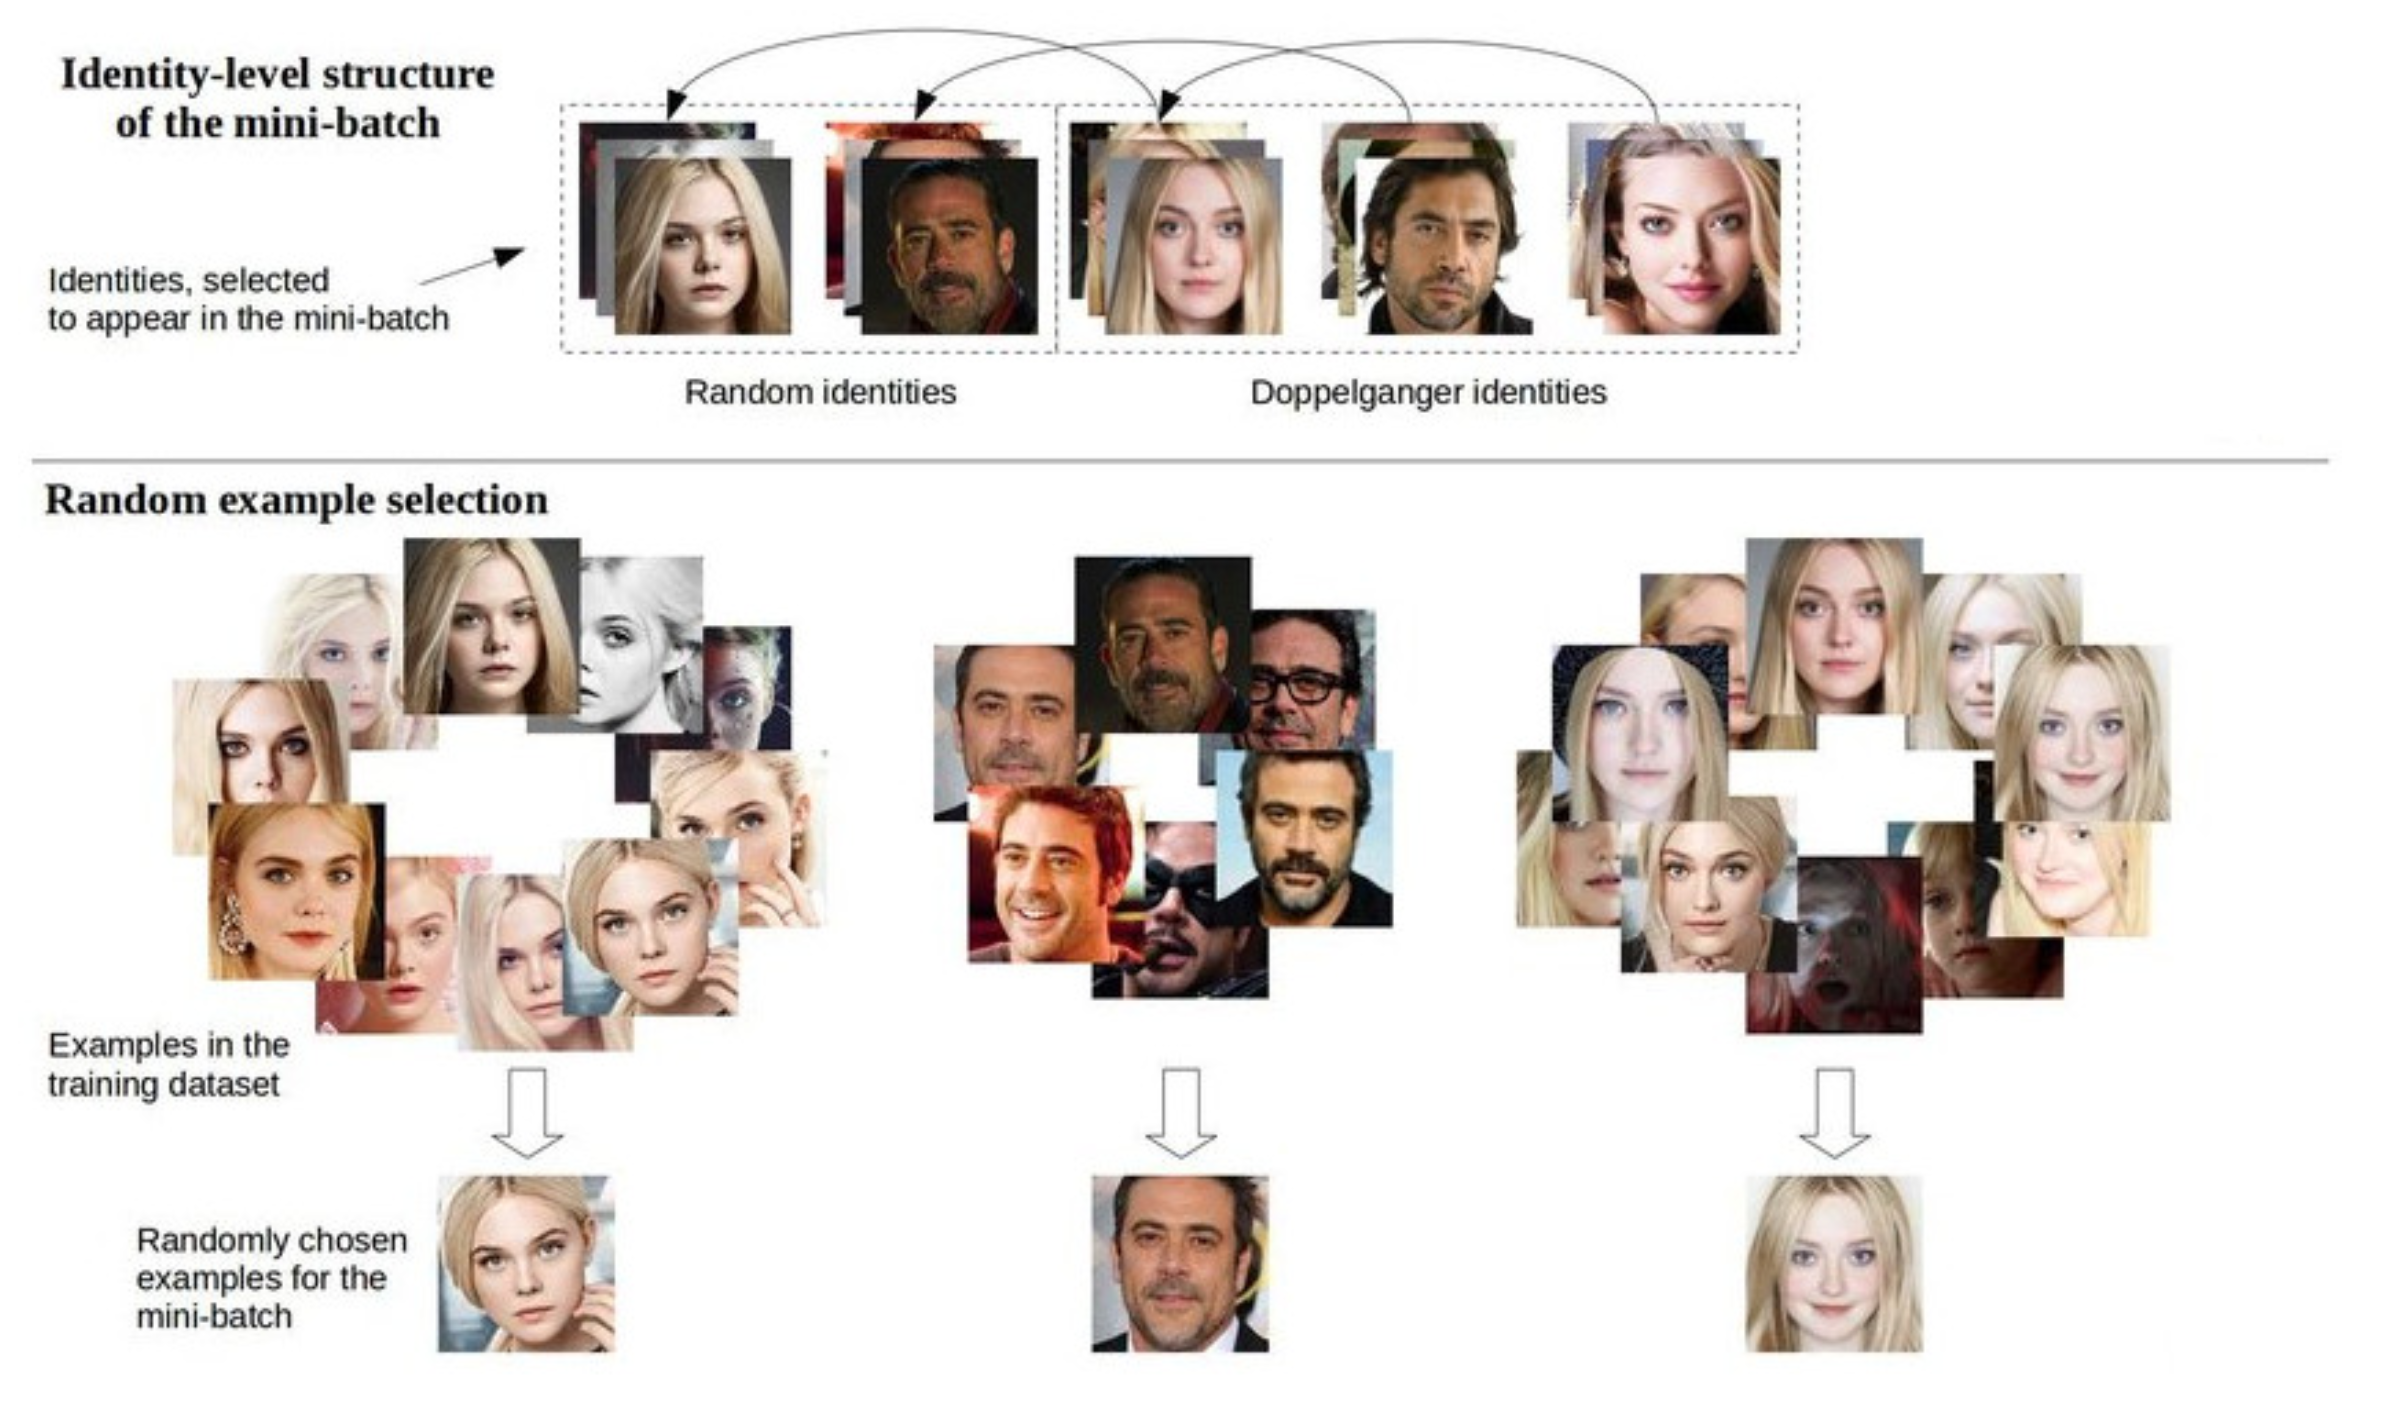
\includegraphics[width=1\linewidth]{img/hardpos_negmin.png}
    
\end{figure}

\begin{itemize}
    \item Mini-batches are composed by selecting identities and their look-alikes to incorporate a range of visual features.
    \item Multiple images for each chosen identity are included to provide variability within the same class.
    \item Random selection from these images ensures that the mini-batch exposes the model to different variations and poses.
\end{itemize}




\subsubsection*{Hard Example Mining}
\begin{figure}[H]
    \centering
    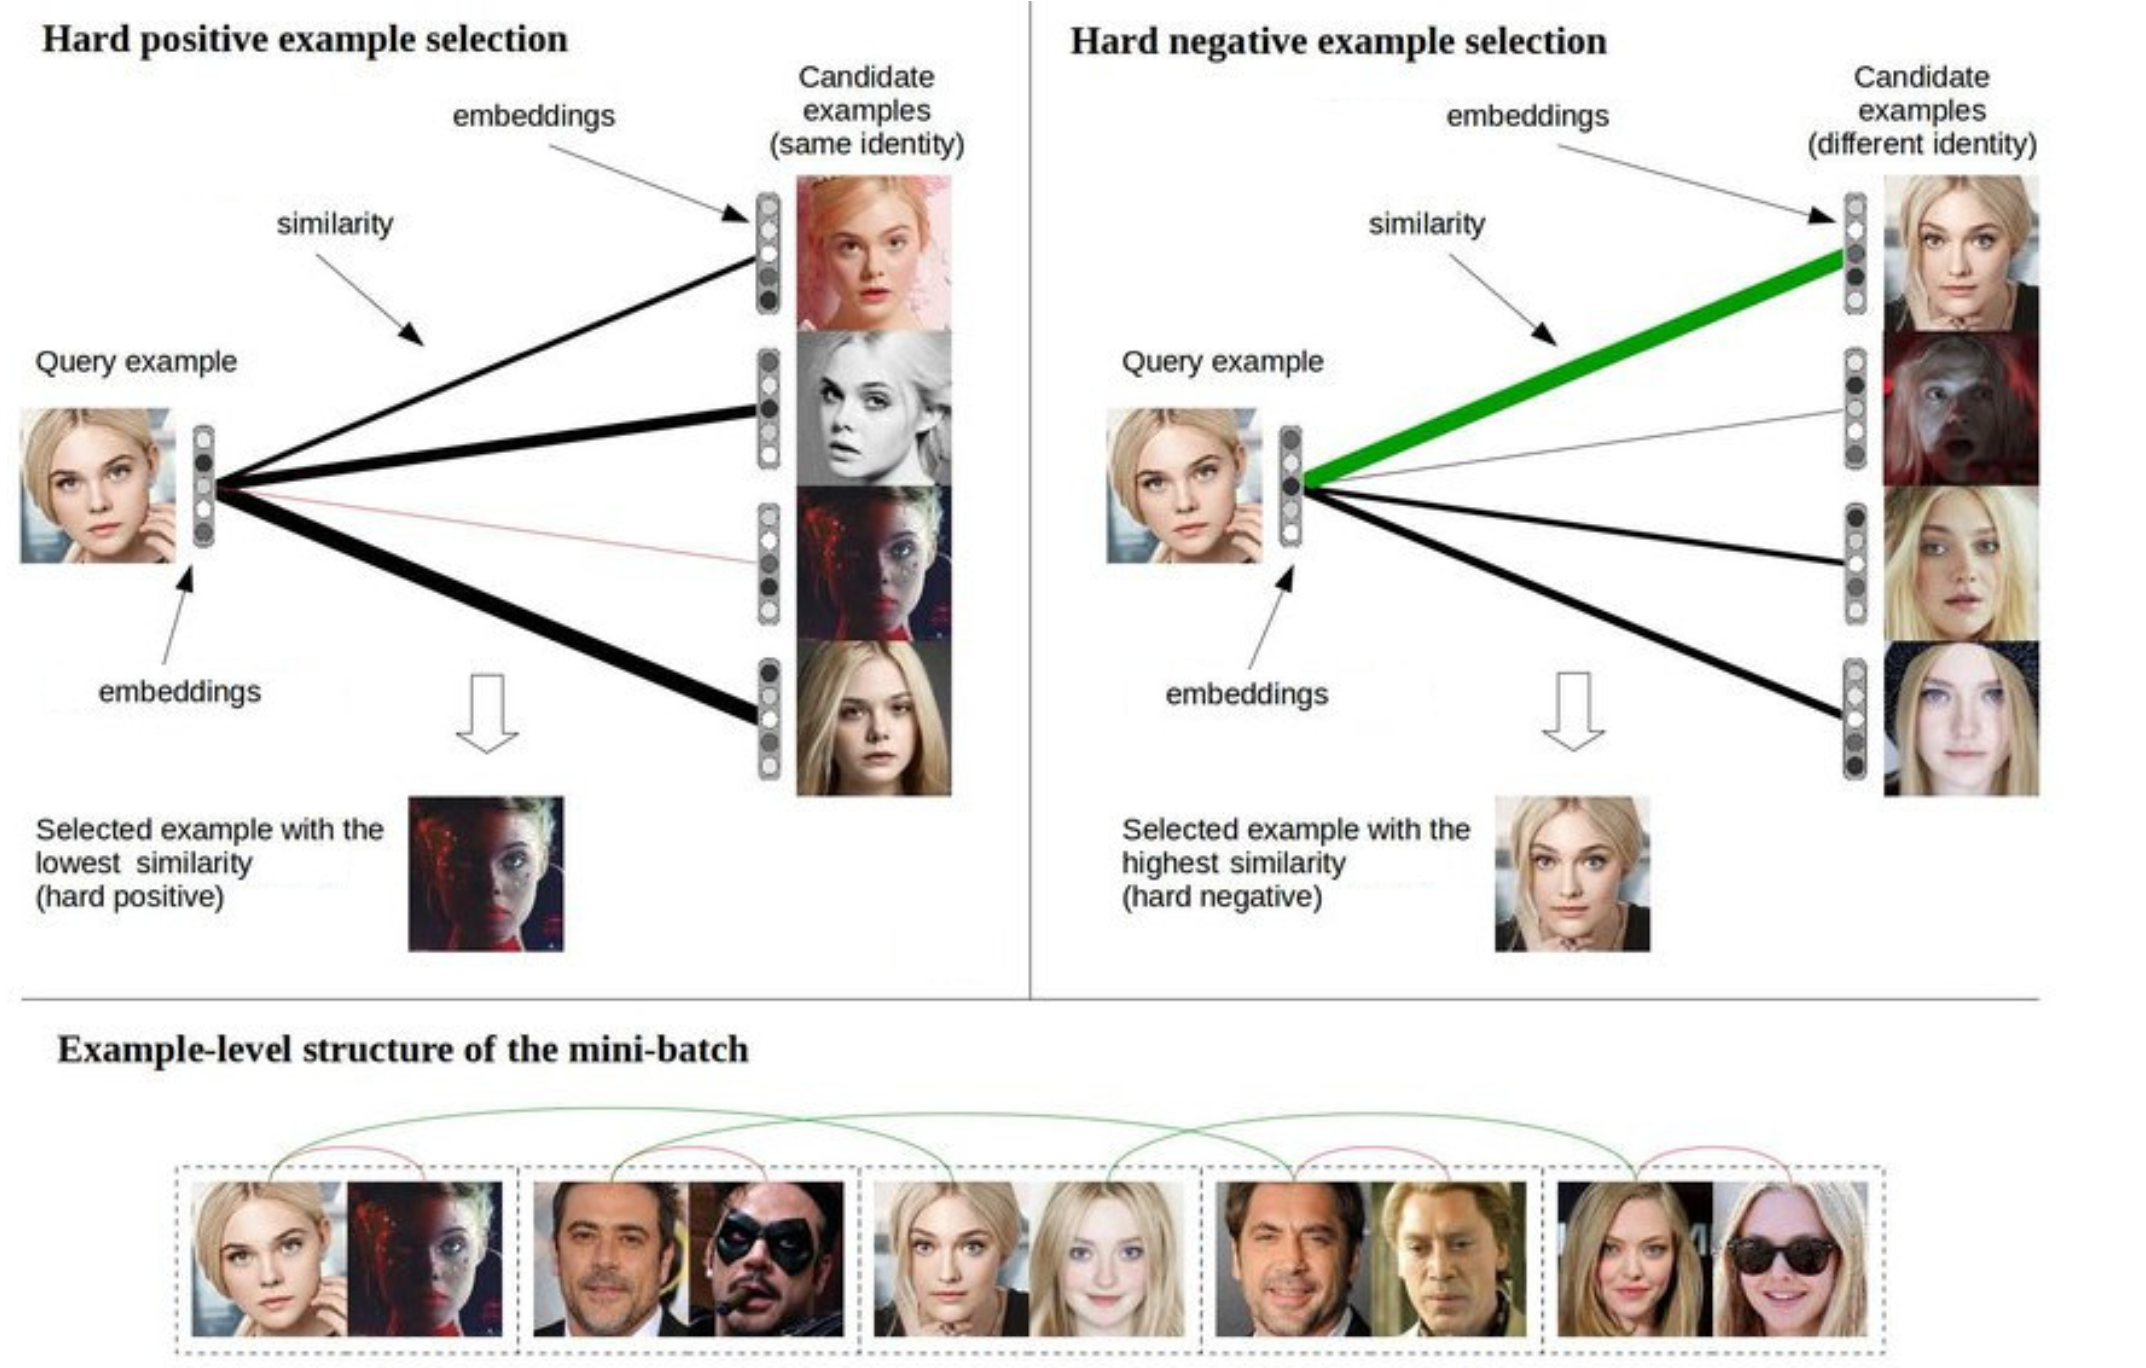
\includegraphics[width=1\linewidth]{img/hardpos_negmin2.png}
\end{figure}


\begin{itemize}
    \item For each query image, hard positives are the least similar images within the same identity class.
    \item Hard negatives are the most similar images from different identity classes.
    \item This selection strategy challenges the model to refine its discriminative abilities.
    \item The final mini-batch is a curated mix of hard positives and negatives to robustly train the model.
\end{itemize}

    
\subsection{Setting Parameters}
\subsubsection*{Hyper-parameters}
\begin{itemize}
    \item Optimising hyper-parameters significantly influences the local minima that the model can attain, correlating with the model's effective capacity.
    \item If encountering memory issues, consider reducing the batch size.
    \item Larger architectures tend to increase the model's capacity, but this is constrained by available memory and computational time.
    \item Decreasing the generalisation gap can be achieved by increasing regularisation measures, such as weight decay and dropout rate.
    \item Data augmentation strategies do not alter model capacity but can improve generalisation.
\end{itemize}

\textbf{Good Rule of Thumb:}
\begin{itemize}
    \item Begin the hyper-parameter tuning process with default parameters.
\end{itemize}

\subsubsection*{Hyper-parameter Search}
\begin{itemize}
    \item Effective hyper-parameter search is often guided by a combination of good intuition and experience.
    \item For learning rate and momentum:
    \begin{itemize}
        \item Gradually decrease the learning rate during training.
        \item Set momentum values typically between 0.8 and 0.9.
    \end{itemize}
    \item Batch Size Considerations:
    \begin{itemize}
        \item Always shuffle the data before batching.
        \item For large datasets, use a batch size that fits your memory constraints.
        \item For smaller datasets, balance instance randomness with gradient smoothness.
    \end{itemize}
    \item Optimise hyper-parameters more efficiently through random search instead of grid search.
    \item Model-based hyper-parameter selection can be effective.
    \item Employ coarse-to-fine searches for hyper-parameters and use a logarithmic scale when appropriate, like for learning rates.
\end{itemize}

\subsection{Monitoring and Debugging}

\subsubsection*{Small Dataset Benchmarks}
\begin{itemize}
    \item Monitor the training error or plot to check if the model is capable of overfitting a small dataset, which is expected behaviour.
    \item Adjust optimisation parameters if the model does not overfit:
    \begin{itemize}
        \item Review the code for potential bugs if adjustments do not lead to overfitting.
    \end{itemize}
    \item Consider reducing the model's size (architecture) if the model compilation time is excessive.
\end{itemize}

\subsubsection*{Hyper-Parameter Optimisation}
\begin{itemize}
    \item Fine-tune hyper-parameters during the validation phase and assess performance on the test set.
    \item Keep a record of both training and validation loss throughout the training period.
    \item Implement early stopping if there is a divergence in training and validation loss trends to prevent overfitting.
    \item Employ patience as a strategy, allowing a certain number of epochs to pass before making significant changes based on improvements.
    \item Assess model performance using multiple metrics as loss alone is not comprehensive; include precision, class-wise precision, and others for a holistic view.
\end{itemize}

\subsubsection*{Model Predictions and Error Analysis}
\begin{itemize}
    \item Verify input data and annotations for correctness.
    \item Confirm that the model predictions are logical and align with expectations.
    \item For error analysis, select a sample of validation set examples where the model has erred.
    \item Manually inspect these examples to understand common error patterns.
    \item Summarise findings in a simple table for clear communication of error types.
\end{itemize}

\subsubsection*{Monitoring Model Internals}
\begin{itemize}
    \item Keep track of histograms of activations and gradient updates per layer to analyse the model's learning behaviour.
    \item Watch for erratic or unstable histogram patterns, which may indicate issues with model training.
    \item Aim for uniform histograms which can be indicative of stable learning dynamics.
\end{itemize}

\begin{figure}[H]
    \centering
    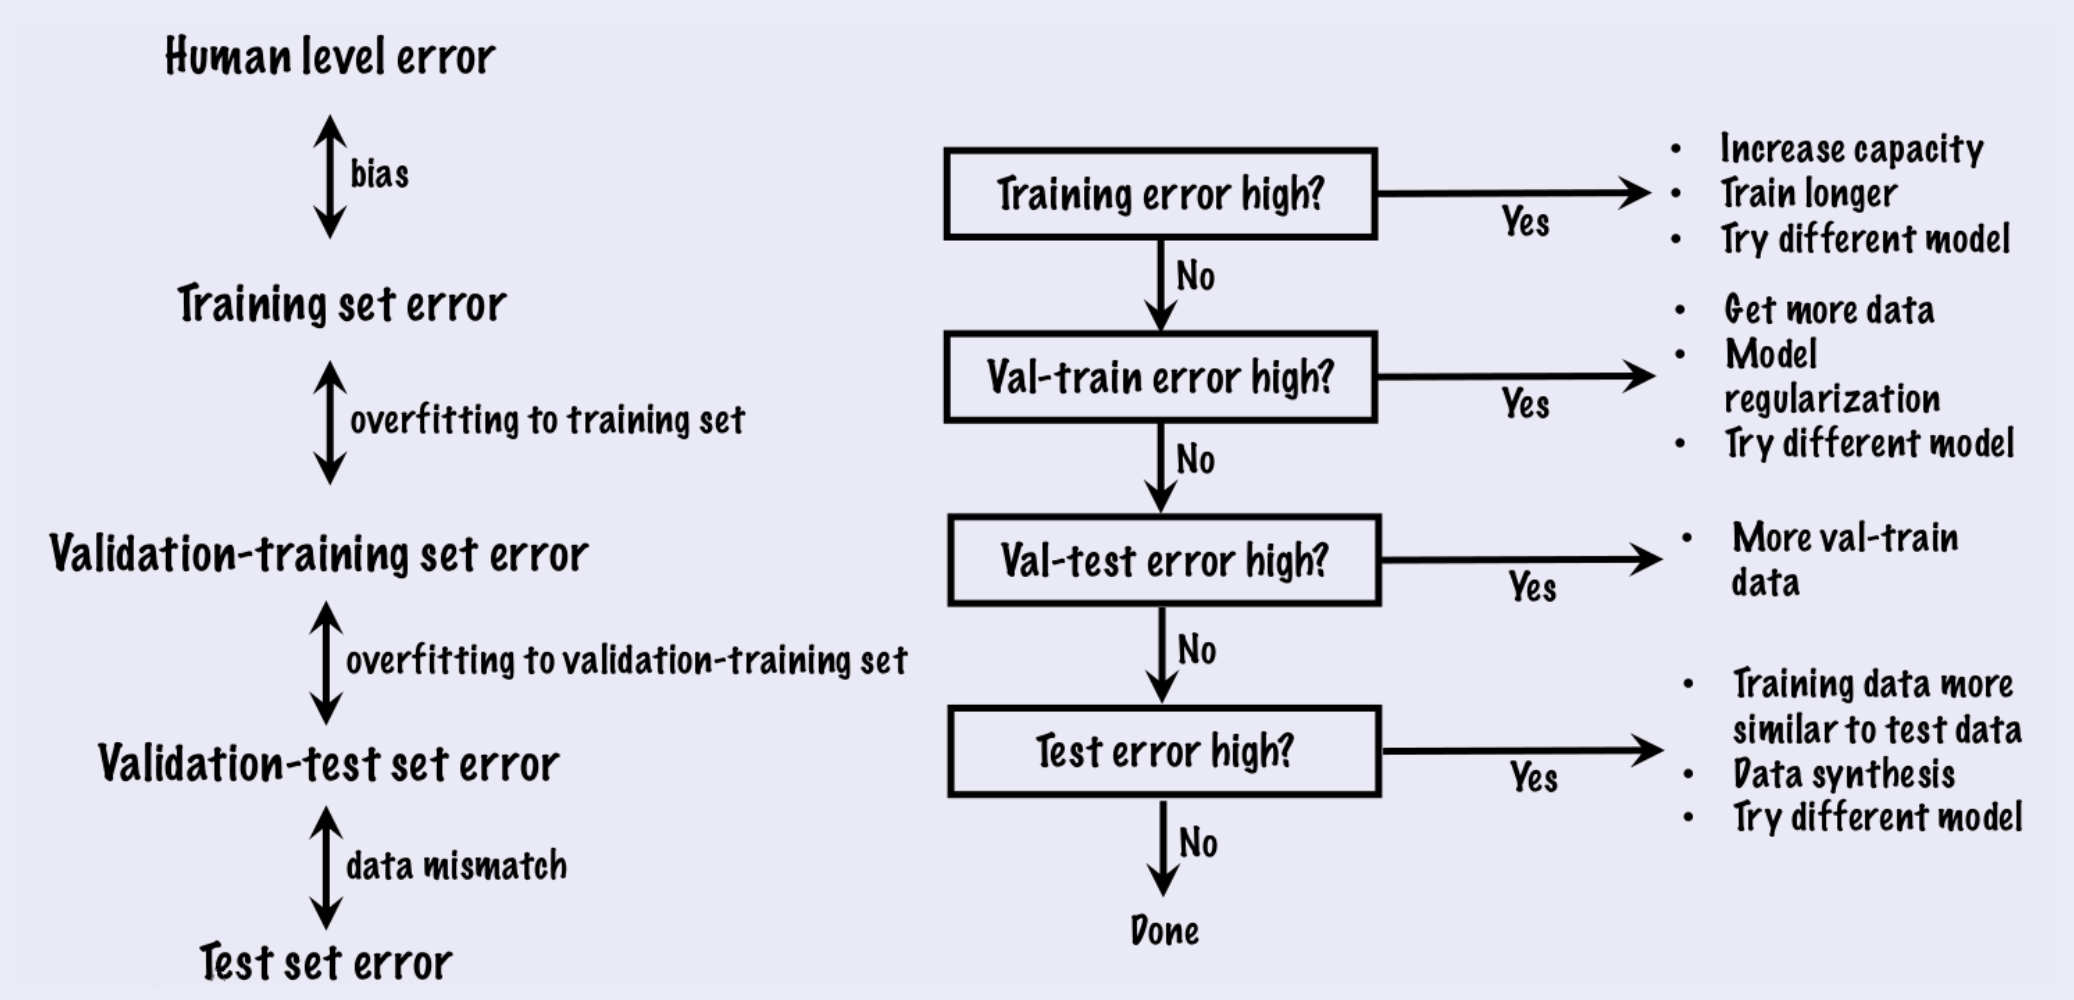
\includegraphics[width=0.75\linewidth]{img/error_analysis.png}
\end{figure}
